% !TeX program = XeLaTeX or LuaLaTeX
% !TeX encoding = UTF-8 Unicode
% Copyright [2021] [Javinator9889]

% Licensed under the Apache License, Version 2.0 (the "License");
% you may not use this file except in compliance with the License.
% You may obtain a copy of the License at

%     http://www.apache.org/licenses/LICENSE-2.0

% Unless required by applicable law or agreed to in writing, software
% distributed under the License is distributed on an "AS IS" BASIS,
% WITHOUT WARRANTIES OR CONDITIONS OF ANY KIND, either express or implied.
% See the License for the specific language governing permissions and
% limitations under the License.
\documentclass[a4paper,oneside,12pt,titlepage,bibliography=totoc]{scrreport}
%%%%%%%%%%%%%%%%%%%%%%%%%%%%%%%%%%%%%%%%%%%%%%%%%%%%%%%%%%%%%%%%%%%%%%%%%%%%%%%%%
%% Packages
%%%%%%%%%%%%%%%%%%%%%%%%%%%%%%%%%%%%%%%%%%%%%%%%%%%%%%%%%%%%%%%%%%%%%%%%%%%%%%%%%
\usepackage{fontspec}
\usepackage[greek,english,spanish]{babel}
\usepackage{multirow}
\usepackage{amsmath}
\usepackage[xetex]{graphicx}
\usepackage{csquotes}
\usepackage{a4wide} %%Smaller margins, more text per page.
\usepackage{longtable} %%For tables that exceed a page width
\usepackage{pdflscape} %%Adds PDF sup­port to the land­scape en­vi­ron­ment of pack­age
\usepackage{caption} %%Pro­vides many ways to cus­tomise the cap­tions in float­ing en­vi­ron­ments like fig­ure and ta­ble
\usepackage{float} %%Im­proves the in­ter­face for defin­ing float­ing ob­jects such as fig­ures and ta­bles
\usepackage[tablegrid,nochapter]{vhistory} %%Vhis­tory sim­pli­fies the cre­ation of a his­tory of ver­sions of a doc­u­ment
\usepackage[nottoc]{tocbibind} %%Au­to­mat­i­cally adds the bib­li­og­ra­phy and/or the in­dex and/or the con­tents, etc., to the Ta­ble of Con­tents list­ing
\usepackage[toc,page]{appendix} %%The ap­pendix pack­age pro­vides var­i­ous ways of for­mat­ting the ti­tles of ap­pen­dices
\usepackage{pdfpages} %%This pack­age sim­pli­fies the in­clu­sion of ex­ter­nal multi-page PDF doc­u­ments in LATEX doc­u­ments
\usepackage[rightcaption]{sidecap} %%De­fines en­vi­ron­ments called SC­fig­ure and SCtable (anal­o­gous to fig­ure and ta­ble) to type­set cap­tions side­ways
\usepackage[printonlyused]{acronym} %%This pack­age en­sures that all acronyms used in the text are spelled out in full at least once. It also pro­vides an en­vi­ron­ment to build a list of acronyms used
\usepackage{layout} %%The pack­age de­fines a com­mand \lay­out, which will show a sum­mary of the lay­out of the cur­rent doc­u­ment
\usepackage{subfig} %%Pro­vides sup­port for the ma­nip­u­la­tion and ref­er­ence of small or ‘sub’ fig­ures and ta­bles within a sin­gle fig­ure or ta­ble en­vi­ron­ment.
\usepackage[toc]{glossaries} %%The glos­saries pack­age sup­ports acronyms and mul­ti­ple glos­saries, and has pro­vi­sion for op­er­a­tion in sev­eral lan­guages (us­ing the fa­cil­i­ties of ei­ther ba­bel or poly­glos­sia).
\usepackage[left,pagewise,modulo]{lineno} %%Adds line num­bers to se­lected para­graphs with ref­er­ence pos­si­ble through the LATEX \ref and \pageref cross ref­er­ence mech­a­nism
\usepackage[colorlinks=false,hidelinks,pdfstartview=FitV,bookmarks=true]{hyperref}%%The hy­per­ref pack­age is used to han­dle cross-ref­er­enc­ing com­mands in LATEX to pro­duce hy­per­text links in the doc­u­ment. 
\usepackage{metainfo}
% \usepackage[pagestyles,raggedright]{titlesec}
\usepackage{etoolbox}
\usepackage{tabularx}
\usepackage{ltxtable}
\usepackage[style=ieee]{biblatex}
\bibliography{base/TFM.bib}
\usepackage[official]{eurosym}
\usepackage{gensymb}
\usepackage{qrcode}
\usepackage{numprint}
\usepackage{mathtools}
\usepackage[nice]{nicefrac}
\usepackage{%
    abstract,
    afterpage,
    array, %%An ex­tended im­ple­men­ta­tion of the ar­ray and tab­u­lar en­vi­ron­ments which ex­tends the op­tions for col­umn for­mats, and pro­vides "pro­grammable" for­mat spec­i­fi­ca­tions
    booktabs, %%The pack­age en­hances the qual­ity of ta­bles in LATEX, pro­vid­ing ex­tra com­mands as well as be­hind-the-scenes op­ti­mi­sa­tion
    dcolumn, %%
    enumitem,
    lastpage,
    lipsum,
    longtable,
    lscape,
    mathcomp,
    microtype,
    pgfplots,
    qtree,
    rotating,
    scrhack,
    scrlayer-scrpage,
    shortvrb,
    skmath,
    titleps,
    titling,
    units,
    url,
    wasysym,
}
%% libertine font for the document body
\usepackage{libertine}
\usepackage[libertine]{newtxmath}

\newcommand{\bigO}[1]{%
  \text{\usefont{OMS}{cmsy}{m}{n}O}\left(#1\right)%
}
%%%%%%%%%%%%%%%%%%%%%%%%%%%%%%%%%%%%%%%%%%%%%%%%%%%%%%%%%%%%%%%%%%%%%%%%%%%%%%%%%
%% Java --> latex 
%%%%%%%%%%%%%%%%%%%%%%%%%%%%%%%%%%%%%%%%%%%%%%%%%%%%%%%%%%%%%%%%%%%%%%%%%%%%%%%%%
\setmonofont{Fira Code}[
  Contextuals=Alternate,
  Ligatures = {Common,Rare}
]
\usepackage{letltxmacro}
\LetLtxMacro\oldttfamily\ttfamily
\DeclareRobustCommand{\ttfamily}{\oldttfamily\csname ttsize\endcsname}
\newcommand{\settttsize}[1]{\def\ttsize{#1}}%
\usepackage{lstfiracode}
\usepackage{listings}

\lstset{ %
  backgroundcolor=\color{white},   % Indica el color de fondo; necesita que se añada \usepackage{color} o \usepackage{xcolor}
  basicstyle=\footnotesize\ttfamily,        % Fija el tamaño del tipo de letra utilizado para el código
  breakatwhitespace=false,         % Activarlo para que los saltos automáticos solo se apliquen en los espacios en blanco
  inputencoding=utf8,
  breaklines=true,                 % Activa el salto de línea automático
  captionpos=b,                    % Establece la posición de la leyenda del cuadro de código
  commentstyle=\color{darkgreen},    % Estilo de los comentarios
  extendedchars=true,              % Permite utilizar caracteres extendidos no-ASCII; solo funciona para codificaciones de 8-bits; para UTF-8 no funciona. En xelatex necesita estar a true para que funcione.
  frame=single,	                   % Añade un marco al código
  keepspaces=true,                 % Mantiene los espacios en el texto. Es útil para mantener la indentación del código(puede necesitar columns=flexible).
  columns=flexible,
  keywordstyle=\color{darkorange},       % estilo de las palabras clave
  numbers=left,                    % Posición de los números de línea (none, left, right).
  numbersep=5pt,                   % Distancia de los números de línea al código
  numberstyle=\small\color{gray}, % Estilo para los números de línea
  rulecolor=\color{black},         % Si no se activa, el color del marco puede cambiar en los saltos de línea entre textos que sea de otro color, por ejemplo, los comentarios, que están en verde en este ejemplo
  showspaces=false,                % Si se activa, muestra los espacios con guiones bajos; sustituye a 'showstringspaces'
  showstringspaces=false,          % subraya solamente los espacios que estén en una cadena de esto
  showtabs=false,                  % muestra las tabulaciones que existan en cadenas de texto con guión bajo
  stringstyle=\color{darkgreen},     % Estilo de las cadenas de texto
  style=FiraCodeStyle,
  identifierstyle=\color{blue},
  tabsize=4,	                   % Establece el salto de las tabulaciones a 2 espacios
  title=\lstname,                   % muestra el nombre de los ficheros incluidos al utilizar
  caption=\lstname,
  literate={á}{{\'a}}1 {é}{{\'e}}1 {í}{{\'{\i}}}1 {ó}{{\'o}}1 {ú}{{\'u}}1 {Á}{{\'A}}1 {É}{{\'E}}1 {Í}{{\'I}}1 {Ó}{{\'O}}1 {Ú}{{\'U}}1 {ü}{{\"u}}1 {Ü}{{\"U}}1 {ñ}{{\~n}}1 {Ñ}{{\~N}}1 {¿}{{?``}}1 {¡}{{!``}}1 {º}{\textdegree}1,
  postbreak=\mbox{\textcolor{red}{$\hookrightarrow$}\space},
}
\lstdefinestyle{C}{%
  language=C,                 % El lenguaje del código
  otherkeywords={__attribute__, __interrupt__, config, inline, asm, uint8_t, uint16_t,%
  uint32_t, uint64_t, time_t, size_t, servo_t, motor_t, Nop,%
  point_t, angle_t, double64_t, int_fast64_t, bool, true, false, stdbool, stdint,%
  stdlib, stddef}           % Si se quieren añadir otras palabras clave al lenguaje
}
\lstdefinestyle{Python}{%
  language=Python
}

\lstdefinestyle{Ada}{%
  language=Ada
}
\lstdefinestyle{bash}{%
  language=bash,
  otherkeywords={sudo,chmod,chown,chgrp,ls,mkdir,touch,useradd,groupadd,usermod}
}
\lstdefinestyle{R}{%
  language=R,
  otherkeywords={0,1,2,3,4,5,6,7,8,9},
  morekeywords={TRUE,FALSE},
  deletekeywords={data,frame,length,as,character}
}
\usepackage{xcolor}
\definecolor{pblue}{rgb}{0.13,0.13,1}
\definecolor{pgreen}{rgb}{0,0.5,0}
\definecolor{pred}{rgb}{0.9,0,0}
\definecolor{pgrey}{rgb}{0.46,0.45,0.48}
\definecolor{darkgreen}{rgb}{0.0, 0.4, 0.0}
\definecolor{darkorange}{rgb}{1.0, 0.55, 0.0}
% \usepackage{inconsolata}
%%%%%%%%%%%%%%%%%%%%%%%%%%%%%%%%%%%%%%%%%%%%%%%%%%%%%%%%%%%%%%%%%%%%%%%%%%%%%%%%%
% \setlength{\parindent}{0pt}
\setlength{\parskip}{.5\baselineskip}
%% Checkmark symbols
\usepackage{pifont}
\newcommand{\cmark}{\ding{51}}%
\newcommand{\xmark}{\ding{55}}%
\newcommand{\done}{\rlap{$\square$}{\raisebox{2pt}{\large\hspace{1pt}\cmark}}%
\hspace{-2.5pt}}
\newcommand{\wontfix}{\rlap{$\square$}{\large\hspace{1pt}\xmark}}

% Greek letters
% \newcommand{\textgreek}[1]{\begingroup\fontencoding{LGR}\selectfont#1\endgroup}

%% Blank pages
\newcommand\blankpage{%
    \null
    \thispagestyle{empty}%
    \addtocounter{page}{-1}%
    \newpage}

%%%%%%%%%%%%%%%%%%%%%%%%%%%%%%%%%%%%%%%%%%%%%%%%%%%%%%%%%%%%%%%%%%%%%%%%%%%%%%%%%
%% Input of the metadata
%%%%%%%%%%%%%%%%%%%%%%%%%%%%%%%%%%%%%%%%%%%%%%%%%%%%%%%%%%%%%%%%%%%%%%%%%%%%%%%%%
\usepackage{environ}
\usepackage[TS1,T1]{fontenc}
\usepackage{graphicx}
\usepackage{array, booktabs, longtable}
\usepackage{caption}
\definecolor{LightSteelBlue3}{rgb}{.64,.71,.8}
\newcommand{\foo}{\color{LightSteelBlue3}\makebox[0pt]{\textbullet}\hskip-0.5pt\vrule width 1pt\hspace{\labelsep}}
\newcommand{\bfoo}{\raisebox{2.1ex}[0pt]{\makebox[\dimexpr2\tabcolsep]%
{\color{LightSteelBlue3}\textbullet}}}%
\newcommand{\tfoo}{\makebox[\dimexpr2\tabcolsep]%
{\color{LightSteelBlue3}$\boldsymbol \uparrow $}}%


\DeclareCaptionFont{blue}{\color{LightSteelBlue3}}
\environbodyname\envbody

\NewEnviron{vtimeline}[2][.9]{%
    \captionsetup{singlelinecheck=false, font=blue, labelfont=sc, labelsep=quad} %
    \begin{longtable}{@{\,}r <{\hskip 2pt} !{\foo} p{#1\linewidth}}%
        \caption{#2} \\[-1.5ex] %
        \toprule
        \addlinespace[2ex]
        \multicolumn{1}{c!{\tfoo}}{}& \\[-2.3ex]
        \envbody
    \end{longtable} %
}

% % Metadaten des Dokumentes

\def\University{\textit{Universidad Politécnica de Madrid}\\ \textit{Escuela Técnica Superior de Ingeniería de Sistemas Informáticos}}
\def\Course{\textit{Máster en Software de Sistemas Distribuidos y Empotrados}}
\def\Module{\textit{Proyecto Fin de Máster}}
\def\Docent{\textit{Tutor: Norberto Cañas de Paz}}
\def\Assistant{}

% pArm -- sistema informático empotrado para gobernar un brazo robótico de diseño abierto
% \def\BoldTitle{\pArm{} --}

\def\Subtitle{VIMS -- \textit{Vehicle IoT Metrics System}}
\def\Authors{Javier Alonso Silva}
\def\Shortname{J. Alonso}


%\Institute\\ \Course\\ \Module\\
% \subject{\Institute \\ \Course \\ \Module}
\title{\Subtitle}
% \title{\Institute\\\Course\\\Module\\\Subtitle}
% \title{\Institute\\ \Course\\ \Module\\ \\ \Subtitle}
\author{\Authors \\ \\ \\ \Docent}
\date{Madrid, \today{}}

%%%%%%%%%%%%%%%%%%%%%%%%%%%%%%%%%%%%%%%%%%%%%%%%%%%%%%%%%%%%%%%%%%%%%%%%%%%%%%%%%
%% Creation of pdf information
%%%%%%%%%%%%%%%%%%%%%%%%%%%%%%%%%%%%%%%%%%%%%%%%%%%%%%%%%%%%%%%%%%%%%%%%%%%%%%%%%
\hypersetup{pdfinfo={
			Title={\Subtitle},
			Author={\Authors},
			Subject={\Module -- \Course}
		}}


%%%%%%%%%%%%%%%%%%%%%%%%%%%%%%%%%%%%%%%%%%%%%%%%%%%%%%%%%%%%%%%%%%%%%%%%%%%%%%%%%
%% Creation of the header
%%%%%%%%%%%%%%%%%%%%%%%%%%%%%%%%%%%%%%%%%%%%%%%%%%%%%%%%%%%%%%%%%%%%%%%%%%%%%%%%%
\patchcmd{\chapter}{plain}{short}{}{} %$ <-- the header on chapter 1
% % workaround
% \makeatletter
% \appto{\appendices}{\def\Hy@chapapp{Appendix}}
% \makeatother
\newpagestyle{long}{%
	\sethead[\thepage][][\chaptername\ \thechapter:\ \chaptertitle]{\chaptername\ \thechapter:\ \chaptertitle}{}{\thepage}
	\headrule
}
\newpagestyle{short}{%
	\sethead[\thepage][][]{}{}{\thepage}
	\headrule
}

\addto\captionsspanish{%
  \renewcommand\appendixname{Anexo}
  \renewcommand\appendixpagename{Anexos}
}

%%%%%%%%%%%%%%%%%%%%%%%%%%%%%%%%%%%%%%%%%%%%%%%%%%%%%%%%%%%%%%%%%%%%%%%%%%%%%%%%%
%% Creation of page-styles
%%%%%%%%%%%%%%%%%%%%%%%%%%%%%%%%%%%%%%%%%%%%%%%%%%%%%%%%%%%%%%%%%%%%%%%%%%%%%%%%%
\setlength{\headheight}{8pt}

\newcolumntype{s}{>{\hsize=.5\hsize\linewidth=\hsize}X}
\newcolumntype{P}[1]{>{\hsize=#1\hsize\linewidth=\hsize}X}
\renewcommand\tabularxcolumn[1]{>{\Centering}m{#1}}
% \newcolumntype{b}{>{\hsize=.75\hsize}X}
\newcommand{\heading}[1]{\multicolumn{1}{c}{#1}}
% \newcolumntype{L}[1]{>{\hsize=#1\hsize\raggedright\arraybackslash}X}%
% \newcolumntype{R}[1]{>{\hsize=#1\hsize\raggedleft\arraybackslash}X}%
\newcolumntype{L}[0]{>{\raggedright\arraybackslash}X}%
% \newcolumntype{C}[1]{>{\hsize=#1\hsize\centering\arraybackslash}X}%
\newcolumntype{C}[1]{>{\Centering\hsize=#1\hsize}X}%

% \usepackage[definemenumacros=false]{menukeys}

\DeclareMathOperator{\atantwo}{atan2}

\DeclareMathOperator{\arctantwo}{arctan2}
%%%%%%%%%%%%%%%%%%%%%%%%%%%%%%%%%%%%%%%%%%%%%%%%%%%%%%%%%%%%%%%%%%%%%%%%%%%%%%%%%
%% DOCUMENT
%%%%%%%%%%%%%%%%%%%%%%%%%%%%%%%%%%%%%%%%%%%%%%%%%%%%%%%%%%%%%%%%%%%%%%%%%%%%%%%%%
\begin{document}
%% Custom listing settings
\settttsize{\footnotesize}
\ActivateVerbatimLigatures

\begin{titlepage}
  \begin{flushleft}
    \includegraphics[width=.4\linewidth]{images/etsisi.png}
  \end{flushleft}
  \begin{center}
    \vspace*{1cm}

    \Huge
    \Course

    \vspace{2cm}
    \huge
    \Subtitle

    \vspace{2cm}

    \LARGE
    \textsc{Proyecto Fin de Máster}

    \vfill

    \Large
    \textit{\Authors}

    \vspace{0.5cm}

    julio de 2022
  \end{center}
\end{titlepage}

\thispagestyle{empty}
\begin{flushleft}
  \includegraphics[width=.4\linewidth]{images/etsisi.png}
\end{flushleft}
\begin{center}
  \vspace*{1cm}

  \Huge
  \Course

  \vspace{2cm}
  \huge
  \Subtitle

  \vspace{2cm}

  \LARGE
  \textsc{Proyecto Fin de Máster}

  \vfill

  \Large
  \begin{flushright}
    \textit{Autor: \Authors} \\
    \textit{Director: \Docent} \\
  \end{flushright}

  \vspace{0.5cm}

  julio de 2022
\end{center}
\newpage


\thispagestyle{empty}
\topskip0pt
\vspace*{\fill}
\begin{flushright}
  \textit{A mi familia, a la banda,\\
    pero sobre todo a mi pareja, \\
    que me ha acompañado en estos momentos \\
    y a Norberto, por su inestimable apoyo y ayuda \\
    (!`ya queda menos para la máquina del tiempo!)}
\end{flushright}
\vspace*{\fill}

\newpage
\afterpage{\blankpage}
%% Include table of contents and history using roman numbering
\pagenumbering{roman}
\DeclareGraphicsExtensions{.pdf,.jpg,.png}
\pagestyle{short}
%%%%%%%%%%%%%%%%%%%%%%%%%%%%%%%%%%%%%%%%%%%%%%%%%%%%%%%%%%%%%%%%%%%%%%%%%%%%%%%%%
%% Table of contents
%%%%%%%%%%%%%%%%%%%%%%%%%%%%%%%%%%%%%%%%%%%%%%%%%%%%%%%%%%%%%%%%%%%%%%%%%%%%%%%%%
\tableofcontents
\listoffigures
\listoftables

\newpage
\pagestyle{long}

%%%%%%%%%%%%%%%%%%%%%%%%%%%%%%%%%%%%%%%%%%%%%%%%%%%%%%%%%%%%%%%%%%%%%%%%%%%%%%%%%
%% Version table insertion
%%%%%%%%%%%%%%%%%%%%%%%%%%%%%%%%%%%%%%%%%%%%%%%%%%%%%%%%%%%%%%%%%%%%%%%%%%%%%%%%%
% \chapter*{Historial de versiones}
\addcontentsline{toc}{chapter}{Historial de versiones}

\begin{table}[H]
  \centering
  \begin{tabularx}{\textwidth}{ |c|c|c|X| }
    \hline
    \textbf{Revisión} & \textbf{Fecha} & \textbf{Autor(es)} & \textbf{Descripción}                                                  \\
    \hline
    0.0               & 28/06/2021     & \Shortname         & Definición de la estructura básica del documento.                     \\
    \hline
    1.0               & 07/07/2021     & \Shortname         & Primera elicitación de requisitos.                                    \\
    \hline
    1.1               & 09/08/2021     & \Shortname         & Añadidos casos de uso en los anexos.                                  \\
    \hline
    1.2               & 08/09/2021     & \Shortname         & Revisión 1.1 realizada junto con el tutor.                            \\
    \hline
    1.3               & 07/03/2022     & \Shortname         & Incluidos diagramas de bloques - segunda revisión junto con el tutor. \\
    \hline
  \end{tabularx}
  \label{tab:hrevision}
\end{table}


\chapter*{Definiciones, siglas, y abreviaturas}
\begin{acronym}
  \acro{ADAS}{\textit{Advanced Driver Assistance Systems}}
  \acro{ADC}{\textit{Analog--Digital Converter}}
  \acro{ALDL}{\textit{Computerized Assembly Line Diagnostics Link}}
  \acro{API}{\textit{Application Programming Interface}}
  \acro{BLE}{\textit{Bluetooth Low Energy}}
  \acro{BR/EDR}{\textit{Basic Rate/Enhaced Data Rate}}
  \acro{CAN}{\textit{Controller Area Network}}
  \acro{CARB}{\textit{California Air Resources Board}}
  \acro{DTC}{\textit{Diagnostic Trouble Codes}}
  \acro{ECU}{\textit{Engine Control Unit}}
  \acro{EOBD}{\textit{European On-Board Diagnostics}}
  \acro{GB}{\textit{gigabyte}}
  \acro{GPIO}{\textit{General Purpose Input/Output}}
  \acro{GPS}{\textit{Global Positioning System}}
  \acro{GUI}{\textit{Graphical User Interface}}
  \acro{IoT}{\textit{Internet of Things}}
  \acro{JOBD}{\textit{Japanese On-Board Diagnostics}}
  \acro{LTE}{\textit{Long--Term Evolution}}
  \acro{MIL}{\textit{Malfunction Indicator Lamp}}
  \acro{MSB}{\textit{Most Significant Bit}}
  \acro{OBD}{\textit{On-Board Diagnostics}}
  \acro{P2P}{\textit{Point-to-Point}}
  \acro{PAN}{\textit{Personal Area Network}}
  \acro{PFM}{Proyecto Fin de Máster}
  \acro{PID}{\textit{Parameter ID}}
  \acro{PWM}{\textit{Pulse--Width Modulation}}
  \acro{RPM}{Revoluciones Por Minuto}
  \acro{SAE}{\textit{Society of Automotive Engineers}}
  \acro{SoC}{\textit{System on Chip}}
  \acro{UART}{\textit{Universal Ascynchronous Receiver--Transmitter}}
  \acro{ULP}{\textit{Ultra Low Power}}
  \acro{VIMS}{\textit{Vehicle IoT Metrics System}}
  \acro{VIN}{\textit{Vehicle Identification Number}}
\end{acronym}

\begin{itemize}
  \item \ac{ADAS} -- sistema de control de un vehículo que utiliza sensores del entorno
        (radar, láser, visión por computador) para mejorar la seguridad al volante y
        la seguridad del entorno ayudando a los conductores a reconocer y reaccionar
        ante eventos o situaciones de tráfico potencialmente peligrosas \cite{hermawanAcquisitionModelingEvaluating2020}.
  \item \ac{API} -- conjunto de definiciones, subrutinas y protocolos que ofrecen
        ciertos \textit{softwares} para ser usados por otras aplicaciones como
        capa de abstracción sobre el original \cite{InterfazProgramacionAplicaciones2021}.
  \item \ac{BLE} -- tecnología \ac{PAN} que permite la comunicación entre dispositivos
        con un rango similar a Bluetooth pero un menor consumo de energía.
  \item \ac{BR/EDR} -- terminología asociada al estándar Bluetooth que define el modo
        de funcionamiento clásico del mismo. Se caracteriza por contar con 79 canales
        de $1~MHz$ de ancho de banda, operar en la red de $2.4~GHz$, ser \ac{P2P},
        transmitir a una velocidad máxima de $3~Mbps$ y tener un consumo medio de
        $1~W$ \cite{ComparisonBluetoothBR}.
  \item Bus \ac{CAN} -- protocolo de comunicaciones de tiempo real para el envío de
        mensajes en entornos distribuidos, permitiendo la comunicación
        entre múltiples CPUs.
  \item \ac{DTC} -- códigos de diagnóstico almacenados en un vehículo que identifican
        un error que tiene el vehículo o que ha tenido.
  \item \ac{ECU} -- centralita electrónica conectado a todos los sensores y sistemas
        del vehículo que recibe la información de los mismos y ejecuta comandos o acciones
        contra ellos.
  \item \ac{GB} -- unidad de almacenamiento de información equivalente a $10^9$ bytes.
  \item \ac{GPIO} -- pin genérico cuyo comportamiento puede ser controlado en tiempo
        de ejecución.
  \item \ac{GPS} -- sistema que permite posicionar cualquier objeto con una 
        precisión de hasta centímetros usando cuatro o más satélites y 
        trilateración \cite{GPS2021}.
  \item \ac{GUI} -- conjunto de componentes visuales que permiten a los usuarios
        interactuar con una aplicación de manera visual e intuitiva.
  \item \ac{IoT} -- concepto que se refiere a la interconexión digital de objetos 
        cotidianos con Internet \cite{InternetCosas2021}.
  \item \textit{jitter} -- retardo relativo que se produce en las comunicaciones
        y que afecta directamente a la saturación de la red y a la capacidad de
        transmisión de la misma.
  \item \ac{LTE} -- también conocido como ``\texttt{4G}'', es la cuarta generación
        del estándar de conexión móvil a Internet que mejora a su predecesor, el \texttt{3G}.
  \item \ac{MSB} -- bit, de acuerdo con su posición, tiene mayor valor (extremo izquierdo).
  \item \ac{OBD} -- sistema de diagnóstico a bordo de vehículos que cuenta con múltiples estándares según la región de uso. Estos
        sistemas ofrecen una monitorización activa y control completo
        sobre el motor y otros dispositivos del vehículo \cite{OBD2021}.
  \item \ac{P2P} -- protocolo de comunicación entre dos nodos en donde sendos nodos se
        interconectan entre sí para el intercambio de información sin necesidad de usar
        un intermediario.
  \item \ac{PAN} -- redes destinadas a la comunicación entre dispositivos en una
        misma red o malla. Tiene un alcance muy limitado, de unos pocos metros por
        lo general.
  \item \ac{PID} -- parámetro utilizado en la comunicación mediante \ac{OBD}--II que
        identifica el tipo de petición que el mecánico/usuario quiera hacer al sistema.
        Son valores enteros de 16 bits que funcionan en formato clave--valor. La información
        devuelta por el conector es también un conjunto de bytes de 32 bits en total que
        representan la información solicitada por el usuario. Por lo general, se deben
        realizar ciertas operaciones aritméticas con ese conjunto de bytes para obtener
        la representación decimal del valor \cite{OBDIIPIDs2021}.
  \item \ac{PWM} -- señal cuadrada de periodo habitualmente constante, entre flancos de
        subida, en la que se modula el tiempo a nivel alto.
  \item \textit{Smog} -- nube baja formada por dióxido de carbono, hollín, humo y polvo
        en suspensión que se forma sobre las grandes ciudades o núcleos industriales.
  \item \ac{SoC} -- denominación asociada a los sistemas (generalmente embebidos) que
        aúnan todos los módulos que requieren para funcionar (y otros tantos para añadir más
        funcionalidades) en un único \textit{chip} que expone al exterior dichas
        funcionalidades mediante una interfaz \textit{hardware} como si fuese un único
        circuito integrado.
  \item trilateración -- método matemático que permite determinar las posiciones
        relativas de objetos usando la geometría de los triángulos \cite{Trilateracion2021}.
  \item \ac{VIN} -- código único, incluyendo el número de serie, que identifica individualmente
        los vehículos a motor, a remolque, motocicletas, \textit{scooters} y \textit{mopeds},
        tal como se define en las ISO 3779 (contenido y estructura) e ISO 4030 (ubicación
        y acoplamiento) \cite{VehicleIdentificationNumber2022}.
\end{itemize}

\addcontentsline{toc}{chapter}{Definiciones, siglas, y abreviaturas}

%% The document itself
%% And reset the numbering as the document starts here
\newpage
\pagenumbering{arabic}
%% Introduction
\begin{abstract}
  En este documento se va a tratar el desarrollo del pArm, un proyecto
  integral de ingeniería en el que se modela, diseña y construye un brazo
  robótico utilizando tecnología de impresión 3D como base. El objetivo
  principal es ofrecer una forma asequible y sencilla para que otra
  persona pueda replicar el proyecto y adentrarse en el mundo de la robótica
  por su cuenta.

  Para ello, primero se elicitarán los requisitos que permitirán posteriormente
  modelar y diseñar el sistema de forma fiel. A su vez, se estudiarán las
  características del sistema \textit{hardware} lo que permitirá desarrollar
  y construir una placa de control que será la encargada de gestionar los
  movimientos del brazo robótico.

  Además, las fases de diseño anteriores simplifican el proceso de desarrollo
  del \textit{software} que ejecutarán los sistemas y permitirán abordar el modelo
  matemático que rige la estructura pantográfica del brazo robótico atendiendo a
  las limitaciones tanto físicas como del sistema propuesto en sí.

  Por otro lado, se modelarán y diseñarán nuevas piezas que permitirán construir el
  brazo robótico con otros tipos de componentes distintos a los del brazo original
  así como con la nueva placa de control.

  Por último, se proponen futuras líneas de mejora que se consideran interesantes
  a la hora de completar el proyecto. Se incluyen además en los anexos el código
  fuente de las aplicaciones desarrolladas ya que se referencia directamente a lo
  largo del presente documento.
\end{abstract}

\selectlanguage{english}
\begin{abstract}
  The pArm development, an integral engineering project which models, designs and
  builds a robotic arm using 3D printing technology as a basis is going. The main objective is to offer an affordable
  and easy way for everyone to replicate this project so they can introduce
  themselves within robotics community.

  Firstly, the requirements will be elicited which, will allow the modeling and the 
  design of the system in further steps of the development. Concurrently, the
  hardware characteristics will be studied in order to allow the development and
  construction of the board that will handle the movements of the robotic arm.

  In addition, the mentioned design steps simplify the software development process
  alongside the mathematical model, which is defined by both the physical structure
  itself and the proposed system.

  On the other hand, new pieces will be designed in order to make the robotic
  manipulator compatible with new external componentes, compared to the 
  original ones used in the $\mu$Arm, and the new designed board.

  Finally, new improvements that the team considers interesting to complete
  will be proposed. The annexes are included with the source code developed for 
  the applications, as they are directly referenced in the present document.
\end{abstract}

\selectlanguage{spanish}


\chapter{Introducción}\label{chap:intro}
En un mundo cada vez más interconectado, hay ciertas tecnologías que se quedan
por detrás en unos campos mientras que siguen progresando en otros. Esto se ve
directamente reflejado en la industria automovilística en donde los vehículos
cada vez cuentan con mayor y mejor tecnología (como cámaras, sensores, actuadores,
etc.) pero no es directamente accesible por el usuario: mediante pantallas e
interfaces se ofrecen métodos sencillos que facilitan su uso.

\ac{VIMS} pretende ser un sistema que facilite el acceso a todos los datos que
ofrece un vehículo para generar estadísticas, descubrir patrones en la conducción
y detectar errores. De esta forma, el conductor tendrá información de primera
mano sobre el estado de su vehículo, eficiencia de su conducción así como obtener
información en tiempo real complementaria a la ya propiciada por el vehículo.

\section{Estado del arte}\label{sec:state_of_the_art}
La historia de la automoción comienza estrictamente en el siglo XIX.
Un automóvil es, por definición, un vehículo que se mueve a sí mismo
(del griego, \textit{αὐτός} ``a sí mismo'' y del latín \textit{mobilis},
``que se mueve'').

Desde los primeros modelos como la serie T, de Ford, hasta el inicio de
la fabricación de vehículos por parte de Mercedes Benz, la historia del
automovilismo ha estado llena de grandes logros y avances en un intervalo
de tiempo relativamente pequeño (figura \ref{fig:ford_model_t}):

\begin{figure}[H]
  \centering
  \includegraphics[width=.8\linewidth]{images/Late_model_Ford_Model_T.jpg}
  \caption{Ford modelo T del 1927 -- de Rmhermen \cite{Ford2022}.}
  \label{fig:ford_model_t}
\end{figure}

Durante aquella época, el ``mejor'' mecanismo de descubrimiento de
problemas era con algunos medidores y, sobre todo, por intuición:
sonidos del motor, olores extraños, \dots

No fue hasta los años 60 en donde los vehículos empezaron a incorporar
distintas interfaces con métricas que podían informar sobre el estado del
vehículo. El gran ``bum'' llegó con la expansión de la computadora, en donde
por primera vez se vio factible introducir un pequeño ordenador de 
abordo en el sistema.

En estos primeros sistemas, se incluyen indicadores del nivel de combustible,
sistema de refrigeración, presión del aceite, velocidad del motor,
temperatura del motor y otra información relativa al combustible. El
primer modelo que se conoce que incluye estos sistemas de cara a la
población en general es el Volkswagen Tipo III, en 1969 (figura \ref{fig:volkswagen_t3}):

\begin{figure}[H]
  \centering
  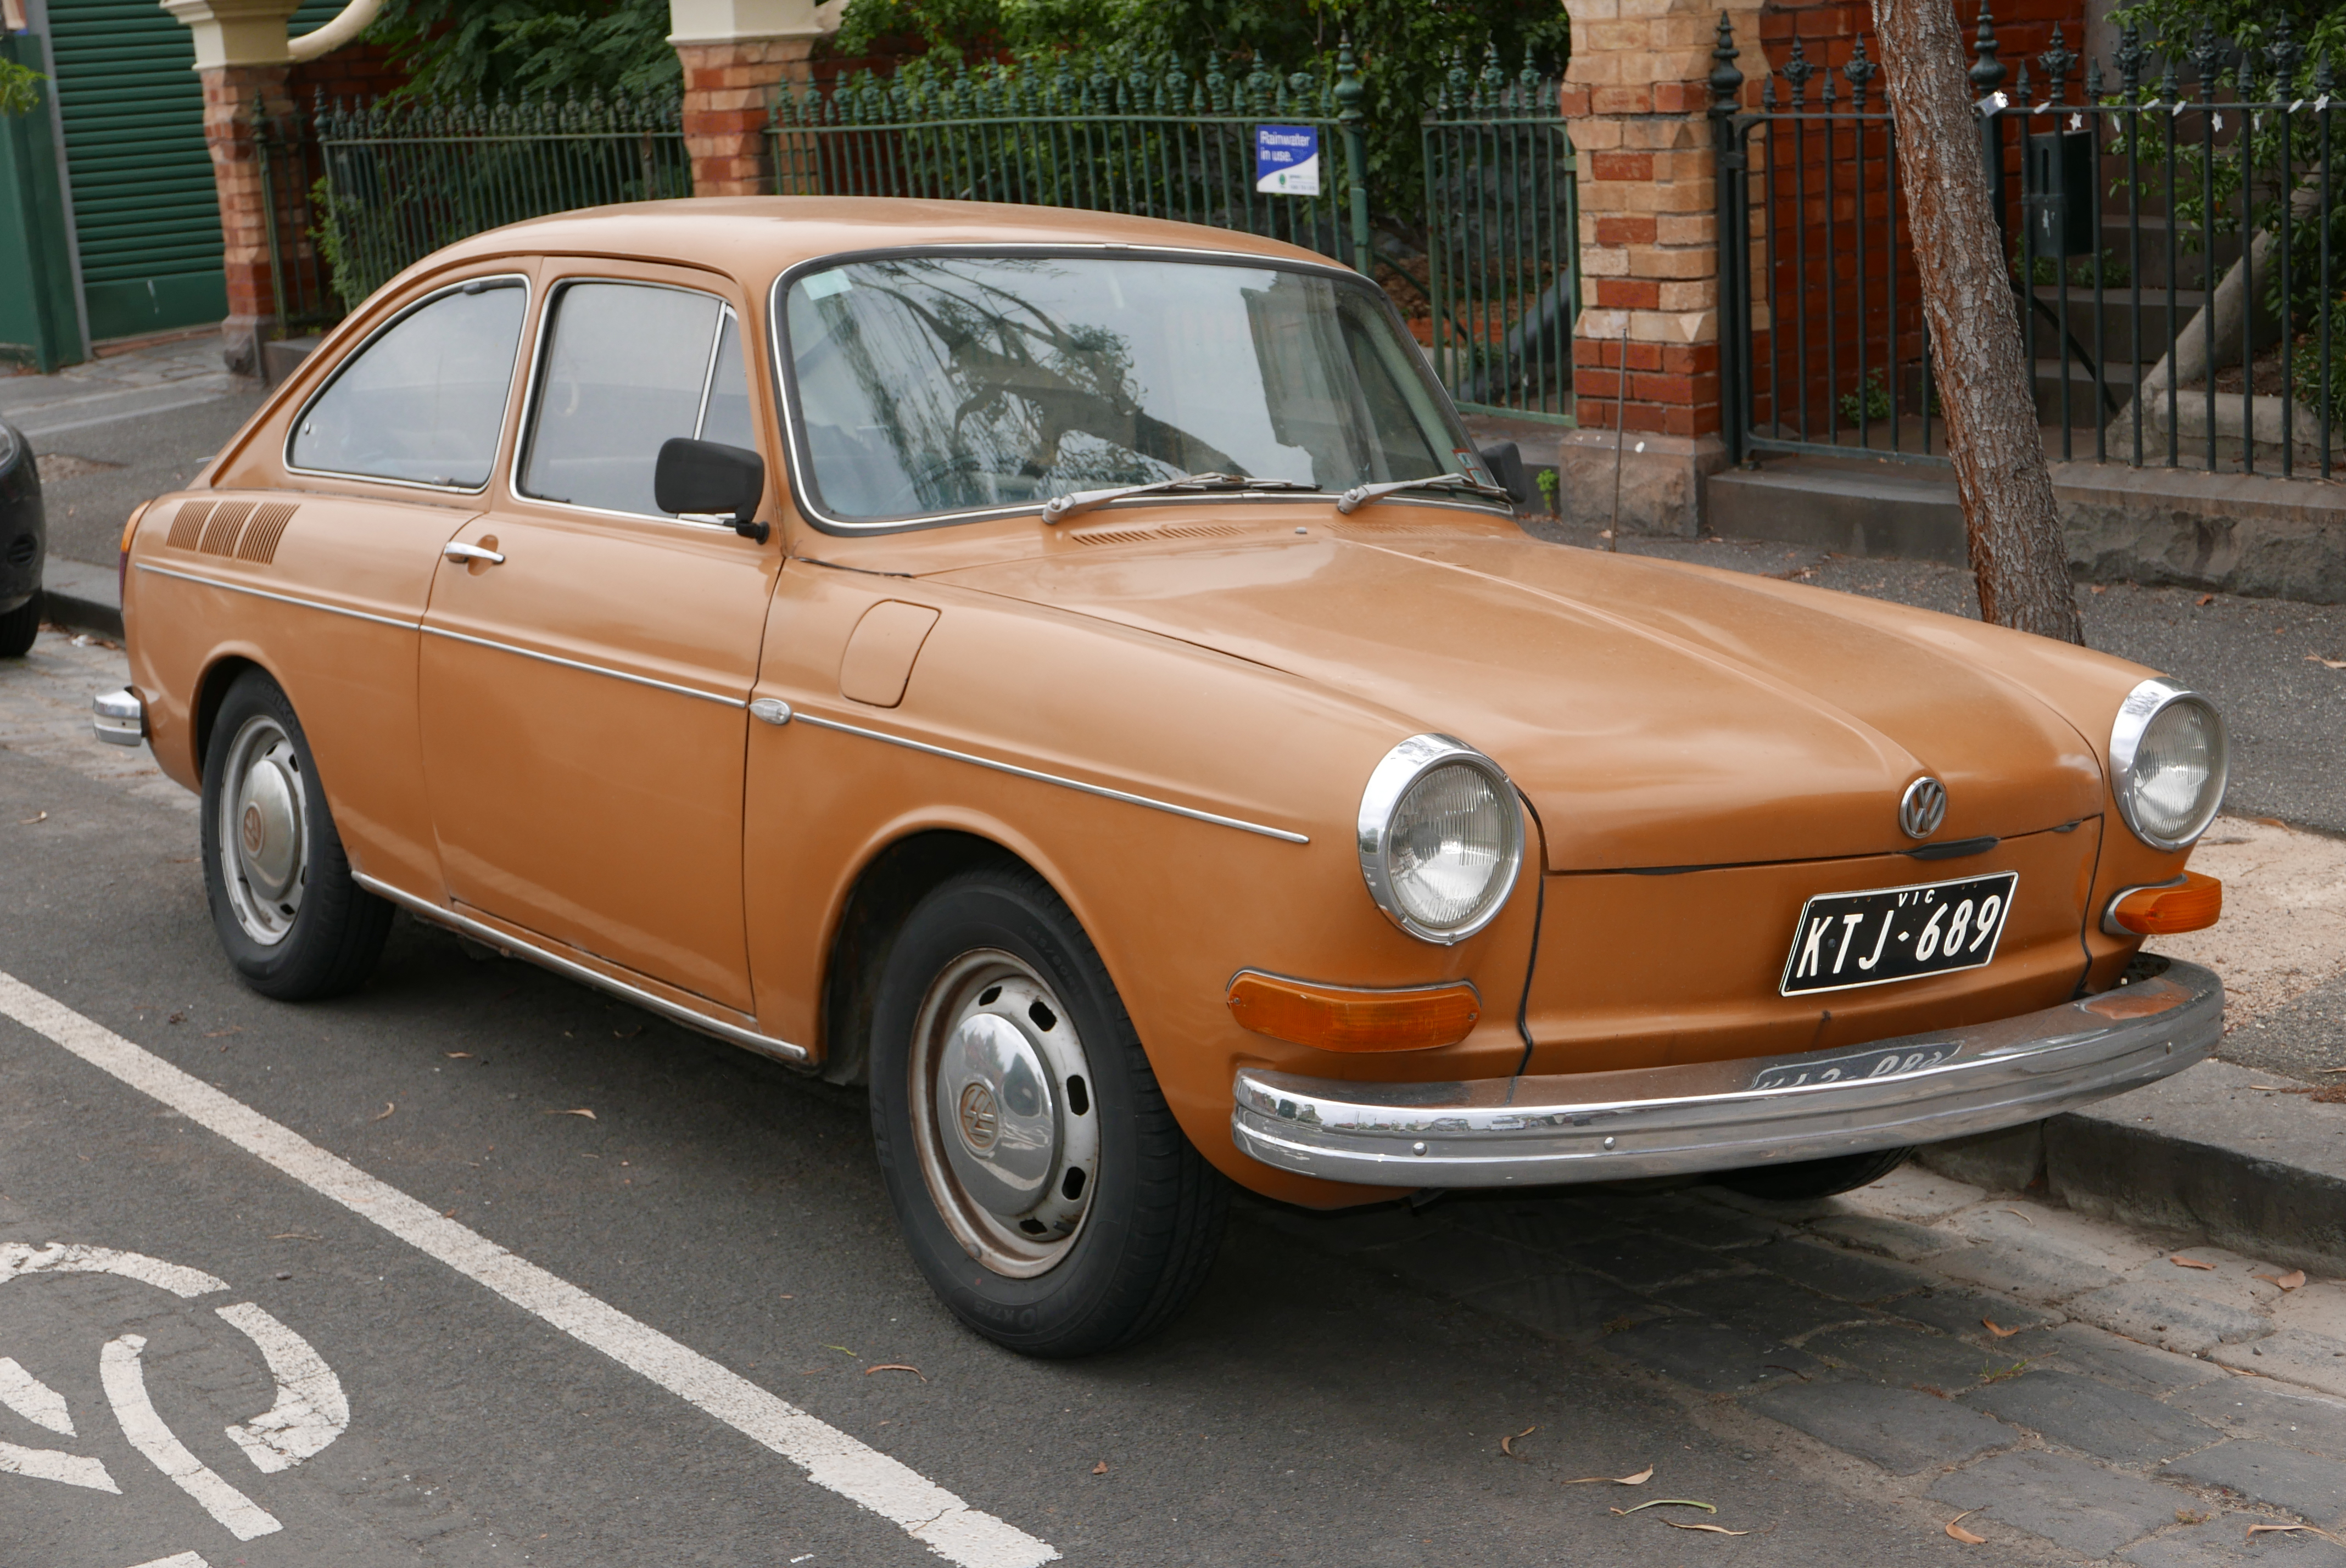
\includegraphics[width=.9\linewidth]{images/volkswagen_t3.jpg}
  \caption{Volkswagen Tipo III, modelo de inyección de 1969 -- de OSX - Trabajo propio \cite{VolkswagenTipo2021}.}
  \label{fig:volkswagen_t3}
\end{figure}

Pese a que supusieron un gran avance, estos primeros sistemas de
diagnóstico daban una información muy valiosa pero limitada, ya que muchos
diagnósticos seguirían siendo mediante los sentidos y las sensaciones
que le transmitiese el vehículo al mecánico. No fue hasta 1980 en donde
se implementó de forma estándar en los vehículos de \textit{General Motors}
el \ac{ALDL}, un lector de errores del coche que funcionó inicialmente a
160 baudios. Años más tarde, el sistema se refinaría usando el estándar
\ac{UART} \textit{half--duplex}, es decir, transmisión en los dos sentidos pero
no de forma simultánea (figura \ref{fig:aldl}). La principal motivación de incluir estos sistemas no fue
otra sino intentar reducir la contaminación de los vehículos teniendo
acceso a esta información \cite{SistemaOBD2Historia}.

\begin{figure}[H]
  \centering
  \includegraphics[width=.75\linewidth]{images/aldl.jpg}
  \caption{Conector \ac{ALDL}, creado por \textit{General Motors} antes de
  estandarizar OBD-II \cite{ReferenceManualChapter}.}
  \label{fig:aldl}
\end{figure}

No es hasta 1979 en que la \ac{SAE} recomienda crear un conector de
diagnóstico estandarizado en el mercado así como un conjunto de señales
de prueba. Finalmente, en 1991 la \ac{CARB} require que todos sus
vehículos tengan lo que sería el \ac{OBD}-I. Esta primera versión informaría
al conductor de un mal funcionamiento de alguno de los elementos del
vehículo mediante un \ac{MIL}, un indicador luminoso de fallos. Sin
embargo, solo se monitorizaban ciertos componentes relacionados con las
emisiones y no estaban calibrados \cite{SistemaOBD2Historia}.

Por ende, impulsado por las alertas \textit{smog} y por una fuerte regulación, en 1994
la \ac{CARB} obligó a todos los vehículos fabricados y vendidos a partir de 1996 incluir
el \ac{OBD}-II. Esto supuso un gran impulso en los mecanismos de monitorización de los
vehículos ya que además se estandarizó tanto el conector como los protocolos recomendados
por la \ac{SAE}. Tiempo más tarde, el Gobierno de los Estados Unidos aplicó la misma
medida a todos los vehículos del país \cite{SistemaOBD2Historia}.

Esta medida llegaría a Europa en 1998, según la Directiva 98/69EG, que obligaba a
todos los vehículos europeos a incluir dicho conector. Específicamente, los
automóviles de gasolina debían empezar a equiparlo en los modelos del año 2000; en el año 2003
para vehículos diésel; y en el año 2005 para camiones \cite{SistemaOBD2Historia}.

\subsection*{OBD--II}
\ac{OBD}--II es la segunda generación del sistema de diagnósticos de abordo, sucesor
de \ac{OBD}--I y su principal función es la de avisar al conductor cuando las
emisiones del vehículo son en torno a $1.5$ veces mayores de las diseñadas. A
diferencia de \ac{OBD}--I, \ac{OBD}--II también detecta fallos eléctricos, químicos
y mecánicos que puedan afectar al nivel de emisiones del vehículo (un caso típico
era un fallo químico del catalizador, indetectable por \ac{OBD}--I pero sí por la
segunda generación).

Este tipo de conector, al ser el primer estándar, cuenta con
múltiples interfaces que permiten conexiones mediante redes Wi-Fi, USB, Bluetooth,
etc. (cayendo pues en deshuso el protocolo de conexión por puerto serie -- RS232).
Esto se ha conseguido gracias al rápido avance de los sistemas embebidos, en donde
la combinación de \textit{software} y \textit{hardware} embebidos ha permitido que
cualquier usuario tenga acceso a este tipo de datos de forma relativamente simple
(actualmente, el conector más estandarizado es el controlador \texttt{ELM327} \cite{SistemaOBD2Historia},
figura \ref{fig:elm327}):

\begin{figure}[H]
  \centering
  \includegraphics[width=.7\linewidth]{images/obd-ii-elm327.jpg}
  \caption{Controlador \texttt{ELM327} que cuenta con antenas Wi-Fi y Bluetooth para un acceso remoto \cite{AmazonComElm327}.}
  \label{fig:elm327}
\end{figure}

El sistema verifica todos los sensores directamente involucrados con las emisiones
del vehículo, como por ejemplo la inyección de aire al motor. Cuando algún sensor detecta
un fallo, se activa el \ac{MIL} indicando el fallo que sucede (o una combinación
de indicadores para notificar la existencia de un fallo, sin especificar exactamente
cuál).

El vehículo que incorpora un conector \ac{OBD}--II almacena la información sobre el
fallo del vehículo para que el mecánico que deba revisar el automóvil disponga de todos
los datos posibles. Por otra parte, este estándar permite una comunicación directa
con el vehículo mediante el envío de órdenes según un \ac{PID}. Por defecto, hay
una serie de \ac{PID}s estándar que la gran mayoría de vehículos deben incluir\footnote{%
Se dice ``la mayoría de vehículos'' porque hay ciertos \ac{PID}s que dependen
directamente del tipo de vehículo (a combustión, eléctrico, \dots) o del combustible
utilizado -- un vehículo eléctrico no ofrece información sobre las \ac{RPM} al igual
que un vehículo diésel no ofrece información sobre las bujías.}, pero también
los fabricantes de vehículos incluyen una serie de \ac{PID}s propios (conocidos como
\textit{\ac{PID}s propietarios}) que ofrecen información adaptada a cada vehículo
en particular y que, en principio, son privados y cerrados al público en general.

En Europa se implantó el \ac{EOBD}, la variación europea del estándar \ac{OBD}--II
implantada en el año 2000 en general. Si bien en apariencia es semejante al \ac{OBD}--II,
las diferencias radican en el \textit{software}. Por ejemplo, el estándar europeo
no monitoriza las evaporaciones del depósito de combustible; sin embargo, es más
sofisticado ya que usa ``mapas'' en las entradas de los sensores que obligan a que el
sensor se calibre empíricamente al sistema según las condiciones de operación del
motor (lo cual se traduce en que los sensores son mucho mejores pero más caros)
\cite{SistemaOBD2Historia}. Otra característica innovadora es que el sistema
europeo registra cuántos kilómetros se han recorrido desde que ha aparecido un
defecto \cite{EOBDOBD2}.

Finalmente, pero no menos importante, Japón tiene también su propio estándar denominado
\ac{JOBD}.

\subsection*{OBD--III}
El \ac{OBD}--III se espera que sea la siguiente versión del sistema que ya implementan
los coches actualmente. La principal diferencia con respecto a la versión anterior
será que el vehículo estará conectado de forma continua y emitiendo datos referentes
a las emisiones. De esta forma, se puede saber casi en el momento acerca de modificaciones
ilegales, un aumento en la contaminación del coche (signo de deterioro) y demás. No se
espera igualmente que sea un salto cualitativo ya que se sigue buscando que sea
altamente compatible con las herramientas que ya existen. Actualmente, se están
realizando pruebas en EE.UU. pero no hay cerrada ninguna fecha de estandarización
oficial por parte de los distintos continentes.

\subsection{Herramientas de monitorización y control del automóvil}
Pese al tiempo que lleva \ac{OBD}--II disponible, las herramientas existentes para
la actuación sobre un vehículo son relativamente escasas. La mayoría de modelos
presentes hoy en día en el mercado se basan directa o indirectamente en el
\texttt{ELM327}, un dispositivo de diagnóstico \ac{OBD} que cuenta con conexión
WiFi, Bluetooth y serie para la lectura local.

Por lo general, las herramientas que hay se utilizan por mecánicos o fanáticos del
sector para acceder a la información del estado del vehículo y ver los errores que
pudiera tener. Sin embargo, tras una breve documentación sobre el tema, la mayoría
de los casos buscaban directamente monitorizar en el momento el estado
del vehículo para obtener información relativa a los consumos, contaminación,
etc.

Por ejemplo, en el trabajo de Rimpas \textit{et al.} \cite{rimpasOBDIISensorDiagnostics2020}, se utiliza
un sensor \texttt{ELM327} para verificar que la información proporcionada por
el puerto del vehículo y la presentada por la telemetría presente en el mismo
(velocímetro y tacómetro) son coherentes entre sí (previa adaptación de los
valores en \textit{bytes} presentados por el conector a valores legibles). En
dicha investigación se llega a la conclusión de que el conector \ac{OBD}--II obtiene
valores fiables y consistentes tanto con los mostrados por el propio vehículo
como los proporcionados por el fabricante.

Otro tipo de investigaciones llevadas a cabo gracias a la presencia de este conector
en los automóviles es la de la caracterización de conductores y hábitos de conducción
según la telemetría reportada por el vehículo. En el estudio realizado por
Galih Hermawan y Emir Husni \cite{hermawanAcquisitionModelingEvaluating2020} se
estudia la combinación de la lectura de los sensores mediante el \ac{OBD}--II con
vehículos que presentan el sistema \ac{ADAS}.
El estudio busca identificar hábitos de conducción según la lectura de los diversos
sensores que hay en el sistema. También persigue detectar quién es el conductor que
está llevando el vehículo actualmente. En el estudio, el uso de \ac{OBD}--II junto
con los algoritmos de los \textit{k--Nearest Neighbor} (k--NN) y \textit{Naive Bayes}
consiguieron una precisión en la identificación del 100\% (
para un conjunto de datos de 10 conductores).
Por otra parte, el uso de inteligencia artificial junto con técnicas de \textit{clustering}
permitieron identificar comportamientos de los conductores al volante y relacionarlo
además con situaciones de riesgo y peligro. Además, se ha aplicado a otras características
también interesantes como detectar el tipo de calzada, predecir el tiempo de viaje,
analizar el consumo del vehículo y demás. El esquema seguido en la investigación es el
que se presenta en la figura \ref{fig:investigation-scheme}:

\begin{figure}[H]
  \centering
  \includegraphics[width=.7\linewidth]{images/general-scheme-investigation.png}
  \caption{Esquema seguido para determinar los hábitos de conducción usando el \ac{OBD}--II \cite{hermawanAcquisitionModelingEvaluating2020}.}
  \label{fig:investigation-scheme}
\end{figure}

Por último, uno de los tipos de investigación bastante interesante realizada en los
últimos años es la de la generación de perfiles de conducción y de consumo. En el
artículo realizado por Ameen \textit{et al.} \cite{husseinaliameenDrivingBehaviourIdentification2021}
se define un sistema de clasificación del comportamiento del conductor al volante
(que es además el que se propone usar en este proyecto) el cual combina los datos
recibidos por el \ac{OBD}--II y del \ac{GPS} (figura \ref{fig:driving-behaviour}):

\begin{figure}[H]
  \centering
  \includegraphics[width=.7\linewidth]{images/driving-behaviour-workflow.png}
  \caption{Flujo de análisis para determinar el comportamiento al volante de un conductor \cite{husseinaliameenDrivingBehaviourIdentification2021}.}
  \label{fig:driving-behaviour}
\end{figure}

Al final, el estudio concluía con los siguientes perfiles de conducción:

\begin{itemize}
  \item \textbf{Peligroso}, para una aceleración en general superior a $7\ \nicefrac{m}{s^2}$.
  \item \textbf{Agresivo}, para una aceleración entre $\left[4\ \nicefrac{m}{s^2}, 7\ \nicefrac{m}{s^2}\right)$.
  \item \textbf{Normal}, para una aceleración entre $\left[2\ \nicefrac{m}{s^2}, 4 \nicefrac{m}{s^2}\right)$.
  \item \textbf{Seguro}, para una aceleración entre $\left[0\ \nicefrac{m}{s^2}, 2\ \nicefrac{m}{s^2}\right)$.
\end{itemize}

\section{Objetivos del desarrollo del proyecto}\label{sec:objectives}
Como se ha podido apreciar, existen multitud de aplicaciones relacionadas directa
o indirectamente con el \ac{OBD}--II, en parte por la longevidad del conector
en el mercado.

Sin embargo, todas o la gran mayoría de aplicaciones están destinadas a los profesionales
del sector, e incluso se ha aprovechado este conector para dificultar el acceso a
los datos del vehículo, habiendo de ir a un taller oficial para que puedan hacer
las reparaciones pertinentes.

Por otra parte, el parque de vehículos español es cada año más viejo debido a
diversos factores que no se van a analizar en este trabajo. Esto implica que cada
año más y más vehículos pierden el soporte por parte del fabricante y se vuelven
cada vez más costosos y complejos de mantener.

Para los no eruditos, el mundo del automóvil es el gran desconocido en donde una
serie de personas cualificadas se encargan del mantenimiento y correcto funcionamiento
del mecanismo que nos transporta por el mundo. Si bien es cierto que es necesaria
esta figura, hay una serie de buenas prácticas y actuaciones que pueden prevenir
tener que ir al mecánico de forma recurrente. Solo hace falta acceso a la información
de manera accesible.

Es por esto que nace \ac{VIMS}, un proyecto que pretende desarrollar un sistema completo
que consta de varias partes: un dispositivo embebido, un servidor y el usuario en sí
(figura \ref{fig:general-scheme}):

\begin{figure}[H]
  \centering
  \includegraphics[width=\linewidth]{images/general-scheme.png}
  \caption{Esquema general que modela el modo de funcionamiento del sistema.}
  \label{fig:general-scheme}
\end{figure}

La idea fundamental detrás de este proyecto es la de devolverle a los usuarios
el control sobre su vehículo, ser conscientes de cómo funciona o, al menos, entender
mejor qué pueden hacer para mejorar tanto su estilo de conducción como la seguridad
al volante. De esta forma, con el dispositivo se espera también prevenir riesgos
ya que los propietarios y usuarios de los vehículos estarán informados en todo
momento de qué error pueda tener.

Como se prevé que este dispositivo sea utilizado por una gran variedad de usuarios
es crucial que sea accesible en términos de sencillez de manejo, entendimiento y
uso: evitar datos excesivamente técnicos, presentar la información más relevante
primero, etc.

Para ello, se hará uso de plataformas en la nube para gestionar, almacenar y presentar
la información al usuario y se contará con una aplicación móvil que permita un
fácil acceso a los datos del vehículo, tanto históricos como generados en el momento.

Al igual que otros trabajos previamente realizados, el proyecto se realiza sobre
las filosofías del código libre y del \textit{hardware} libre, que se traduce en
que todos los recursos (tanto físicos como \textit{software}) estarán disponibles
enteramente para cualquier persona interesada en ver cómo funciona, replicar el
proyecto por su cuenta y contar con plena potestad para mejorarlo, redistribuirlo
y trabajar con él (siempre bajo un prisma de reconocimiento al autor original
del trabajo regido por \textit{copyright}). Para ello, se ha decidido hacer uso
de la licencia MIT\footnote{Se pueden obtener más detalles sobre la licencia MIT
en la siguiente URL: \url{https://choosealicense.com/licenses/mit/}}.

\section{Metodología}\label{sec:methodology}
El proyecto que se pretende desarrollar es un proyecto de ingeniería. Esto se
traduce en que la metodología y la forma de trabajo son pilares fundamentales
en el desarrollo del mismo.

El primer paso realizado fue el de recopilar recursos e información de qué
necesitaban específicamente los usuarios. Para ello, se elaboró un cuestionario
en donde de forma general se preguntaba a conductores y no conductores qué querrían
tener en su vehículo. Los primeros sirvieron como fuente de información principal,
debido a sus características \textit{per se}; los segundos para aumentar la entropía
de los datos obtenidos y usando sus respuestas como grupo de control para validar la
de los primeros. El primer análisis realizado se detalla
en la sección \ref{ssec:user-req}, de la especificación de requisitos. Posteriormente,
en el punto \ref{sec:merch} se analiza en mayor profundidad los datos obtenidos
y se extraerán conclusiones.

A continuación, se realizó un estudio sobre qué plataformas y dispositivos están
accesibles de forma global para la generación y transmisión de datos. Esta fase
se centró principalmente en ``descubrir'' variantes del modelo ESP32 que incluyesen
ciertas antenas para permitir una mayor conectividad. Tras valorar diversas opciones,
se decidió usar el LILYGO T-SIM7000G ESP32 que incluye soporte de forma nativa para
tarjetas microSD, antena \ac{LTE}, alimentación externa por batería, antena \ac{GPS}, WiFi y
Bluetooth.

Una vez se decidió que dispositivo físico se iba a utilizar, se comenzó con el desarrollo
de los distintos diagramas que modelan el sistema, tanto lógicos como de diseño. Esta
parte fue crucial para asentar las bases de lo que será el proyecto y ha permitido seguir
el avance del mismo.

Por último, se realizó el serigrafiado de la placa y se comenzó la implementación
física de los diseños realizados. Por diversos contratiempos que han surgido, el proyecto
se ha planteado finalmente como proyecto de especificación y diseño, con una batería
de ensayos específicos reales que facilitarán la construcción que se va a realizar
posteriormente.


%% Product description
\chapter{Estructura del proyecto}\label{chap:structure}
El desarrollo del sistema \ac{VIMS} es un proceso multidisciplinar en el que se deben
desarrollar varias áreas de conocimiento. Este proyecto se ha postulado como
un desarrollo integral de ingeniería y es por eso por lo que está dividido en
varios bloques que conforman un factor clave en el desarrollo del mismo.

Estas secciones están bien diferenciadas y se conforman de: un estudio de mercado y de
las características de los usuarios, un estudio matemático asociado a la lectura de
valores y adecuación del \textit{hardware}, el proceso de diseño \textit{hardware}
en sí, el diseño \textit{software} del sistema y el análisis de planificación del mismo.

\begin{itemize}
  \item El estudio de mercado pretende averiguar y formalizar las necesidades de los
  conductores y usuarios de la vía. Es la primera aproximación y facilita la
  delimitación del producto y, sobre todo, ofrecerle al usuario final algo de utilidad
  y que pueda necesitar.
  \item El estudio matemático se encarga de investigar la ``traducción'' de los
  valores recibidos por el vehículo (según los datos asociados al estudio de mercado
  realizado con anterioridad).
  \item El diseño \textit{software} modela principalmente cómo se va a estructurar
  el sistema y cómo debe comportarse ante los distintos eventos que puede recibir.
  Esta fase conlleva realizar diagramas lógicos y de diseño del sistema en su conjunto.
  \item El diseño \textit{hardware} conlleva tanto el estudio de los componentes del
  sistema así como de las restricciones físicas del mismo.
  \item El análisis de planificabilidad complementa el diseño \textit{software}
  y estudia si el sistema es planificable. En los requisitos no se define \ac{VIMS}
  como un sistema en tiempo real, pero la cantidad de componentes que contiene y las
  acciones que tiene que realizar requieren del uso de subrutinas y de una planificación
  previa para asegurar un correcto funcionamiento del mismo.
\end{itemize}

Es importante detallar que pese a que el sistema se compone de varios componentes,
son dos los principales que lo caracterizan:

\begin{enumerate}
  \item La placa, \ac{VIMS}, que va embebida en los vehículos del sistema. Se encarga
  de toda la lectura, adaptación y emisión de datos. Además, cuenta con soporte para
  poder realizar una transmisión de la información a un dispositivo asociado mediante
  redes \ac{PAN}.
  \item El servidor \textit{cloud}, el ``cerebro'' encargado de recibir las tramas,
  los datos y la información relativa a las placas \ac{VIMS}, los dispositivos de
  usuario y demás componentes. Además, tiene la responsabilidad de ofrecer a los
  usuarios una \ac{GUI}, generar información relevante a partir de los datos (como
  estadísticas), gestionar las suscripciones y enviar periódicamente la información
  al usuario.
\end{enumerate}

\section{Estudio de mercado}\label{sec:merch}
Para el desarrollo de este proyecto, se hizo un estudio de mercado tanto de los
consumidores como de sus características, además de una evaluación exhaustiva
de qué les gustaría tener en su vehículo.

Este proyecto pretende en un futuro salir a mercado y suplir características que los
usuarios echan en falta en sus correspondientes medios de transporte. Como en principio
funciona con cualquier vehículo que cuente con \ac{OBD}--II, las respuestas no se han
limitado a aquellos conductores que condujesen turismos sino cualquier tipo de
automóvil: motocicleta, camión, etc.

Es importante destacar que el estudio tiene varios sesgos que han restringido
y delimitado las respuestas que se han registrado:

\begin{enumerate}
  \item Se ha realizado un cuestionario usando Google Forms, una plataforma de Google
        que permite preparar una serie de preguntas y respuestas y aplicar ciertos
        filtros sobre ellas. Por ejemplo, para aquellos que dijeron ser conductores,
        se hicieron preguntas diferentes frente a quienes no lo fueran.

        Esto permite obtener datos más fidedignos y acotados según la población que
        respondiera. Sin embargo, tiene una limitación implícita: restringe el acceso
        a aquellos con conocimientos ``suficientes'' acerca de la plataforma. Pese
        a que el producto pretende ser lo más accesible posible, no hy que olvidar
        que este tipo de tecnologías permanecen desconocidas para una gran parte
        de la población con escasos conocimientos acerca de Internet o de las
        nuevas tecnologías. Se comentará más adelante, pero esto se ve reflejado
        principalmente en la edad media de quienes respondieron el cuestionario.

        Por otra parte, al ser un cuestionario aparece otra limitación implícita
        y es la validación y verificación de las respuestas.
\end{enumerate}

\section{Estudio matemático}\label{sec:maths}
El estudio matemático va muy ligado al punto anterior (\ref{sec:merch}) ya que se
analizan los parámetros de \ac{OBD}--II y su ecuación matemática para obtener un
valor en $\mathbb{R}$ entendible por las personas.

Antes de dar paso a las ecuaciones en sí, es importante entender cómo funciona
el conector \ac{OBD}--II en esta situación. Los datos enviados y recibidos por
el coche están siempre codificados en un valor binario, recogido en un vector
de cuatro elementos en donde cada elemento tiene un \textit{byte} de tamaño. De
esta forma, se define al valor obtenido tras leer el conector \ac{OBD}--II como:

\begin{table}[H]
  \centering
  \resizebox{\textwidth}{!}{\begin{tabular}{|c|c|c|c|c|c|c|c|c|c|c|c|c|c|c|c|c|c|c|c|c|c|c|c|c|c|c|c|c|c|c|c|}
      \hline
      \multicolumn{8}{|c|}{$A$} & \multicolumn{8}{|c|}{$B$} & \multicolumn{8}{|c|}{$C$} & \multicolumn{8}{|c|}{$D$}                                                                                                                                                                                                                                 \\
      \hline
      $A_7$                     & $A_6$                     & $A_5$                     & $A_4$                     & $A_3$ & $A_2$ & $A_1$ & $A_0$ & $B_7$ & $B_6$ & $B_5$ & $B_4$ & $B_3$ & $B_2$ & $B_1$ & $B_0$ & $C_7$ & $C_6$ & $C_5$ & $C_4$ & $C_3$ & $C_2$ & $C_1$ & $C_0$ & $D_7$ & $D_6$ & $D_5$ & $D_4$ & $D_3$ & $D_2$ & $D_1$ & $D_0$ \\
      \hline
    \end{tabular}}
  \caption{Vector de \textit{bytes} que representa los datos recibidos del conector \ac{OBD}--II \cite{OBDIIPIDs2021}.}
  \label{tab:byte-array}
\end{table}

De esta forma, cuando se escribe $A_4$ se hace referencia al cuarto bit
del vector $A$. Los bits están ordenados según \ac{MSB}, de forma que
$A_7$ es el bit más significativo y $A_0$ el menor.

Los datos se obtienen del \ac{OBD}--II utilizando un lenguaje estándar llamado
\ac{PID}. El \ac{PID} se codifica como un número entero de 16 bits en donde los 8
primeros bits identifican el servicio/modo y los 8 restantes la operación a realizar.
Actualmente, están registrados los siguientes modos de funcionamiento (tabla
\ref{tab:pids-mode}):

\begin{table}[H]
  \centering
  \begin{tabularx}{\textwidth}{ | c | X | }
    \hline
    \textbf{Modo (hex)} & \textbf{Descripción}                                                                       \\
    \hline
    \texttt{01}         & Muestra los datos actuales del vehículo                                                    \\
    \hline
    \texttt{02}         & Muestra los datos almacenados del cuadro del vehículo                                      \\
    \hline
    \texttt{03}         & Muestra los códigos \ac{DTC}                                                               \\
    \hline
    \texttt{04}         & Elimina los códigos \ac{DTC} almacenados                                                   \\
    \hline
    \texttt{05}         & Resultados del test del sensor de oxígeno (sin \ac{CAN})                                   \\
    \hline
    \texttt{06}         & Resultados del test del sensor de oxígeno (con \ac{CAN})                                   \\
    \hline
    \texttt{07}         & Muestra los códigos \ac{DTC} pendientes (eliminados durante el último ciclo de conducción) \\
    \hline
    \texttt{08}         & Operaciones de control sobre los componentes del sistema                                   \\
    \hline
    \texttt{09}         & Petición de información sobre el vehículo                                                  \\
    \hline
    \texttt{0A}         & Códigos \ac{DTC} eliminados                                                                \\
    \hline
  \end{tabularx}
  \caption{Lista de modos de funcionamiento del estándar \ac{OBD}--II \cite{OBDIIPIDs2021}.}
  \label{tab:pids-mode}
\end{table}

Es importante destacar que no todos los fabricantes tienen por qué soportar todos
los modos, y que además ciertos fabricantes pueden definir sus modos propios por encima
del valor \texttt{09}.

Todos los modos definidos anteriormente tienen un conjunto de órdenes de soporte
en donde el sistema indica qué \ac{PID}s están soportados y cuáles no, por cada 32
\ac{PID}s. Por ejemplo, enviar la orden \texttt{0x0100} (\textit{modo 1, PID 0})
devolverá un valor que representará si los siguientes 32 \ac{PID}s están soportados.
Si el valor fuese, por ejemplo, \texttt{BE1FA813} se tendría que:

\begin{table}[H]
  \centering
  \resizebox{\textwidth}{!}{\begin{tabular}{ | c | c | c | c | c | c | c | c | c | c | c | c | c | c | c | c | c | c | c | c | c | c | c | c | c | c | c | c | c | c | c | c | c | }
      \hline
      \textbf{Hexadecimal} & \multicolumn{4}{|c|}{\texttt{B}} & \multicolumn{4}{|c|}{\texttt{E}} & \multicolumn{4}{|c|}{\texttt{1}} & \multicolumn{4}{|c|}{\texttt{F}} & \multicolumn{4}{|c|}{\texttt{A}} & \multicolumn{4}{|c|}{\texttt{8}} & \multicolumn{4}{|c|}{\texttt{1}} & \multicolumn{4}{|c|}{\texttt{3}}                                                                                                                                                                                                                                                                                                                                                 \\
      \hline
      \textbf{Binario}     & \texttt{1}                       & \texttt{0}                       & \texttt{1}                       & \texttt{1}                       & \texttt{1}                       & \texttt{1}                       & \texttt{1}                       & \texttt{0}                       & \texttt{0}  & \texttt{0}  & \texttt{0}  & \texttt{1}  & \texttt{1}  & \texttt{1}  & \texttt{1}  & \texttt{1}  & \texttt{1}  & \texttt{0}  & \texttt{1}  & \texttt{0}  & \texttt{1}  & \texttt{0}  & \texttt{0}  & \texttt{0}  & \texttt{0}  & \texttt{0}  & \texttt{0}  & \texttt{1}  & \texttt{0}  & \texttt{0}  & \texttt{1}  & \texttt{1}  \\
      \hline
      \textbf{¿Soportado?} & \done                            & \wontfix                         & \done                            & \done                            & \done                            & \done                            & \done                            & \wontfix                         & \wontfix    & \wontfix    & \wontfix    & \done       & \done       & \done       & \done       & \done       & \done       & \wontfix    & \done       & \wontfix    & \done       & \wontfix    & \wontfix    & \wontfix    & \wontfix    & \wontfix    & \wontfix    & \done       & \wontfix    & \wontfix    & \done       & \done       \\
      \hline
      \textbf{PID}         & \texttt{01}                      & \texttt{02}                      & \texttt{03}                      & \texttt{04}                      & \texttt{05}                      & \texttt{06}                      & \texttt{07}                      & \texttt{08}                      & \texttt{09} & \texttt{0A} & \texttt{0B} & \texttt{0C} & \texttt{0D} & \texttt{0E} & \texttt{0F} & \texttt{10} & \texttt{11} & \texttt{12} & \texttt{13} & \texttt{14} & \texttt{15} & \texttt{16} & \texttt{17} & \texttt{18} & \texttt{19} & \texttt{1A} & \texttt{1B} & \texttt{1C} & \texttt{1D} & \texttt{1E} & \texttt{1F} & \texttt{20} \\
      \hline
    \end{tabular}}
  \caption{Obtención de los \ac{PID}s soportados según el modo \cite{OBDIIPIDs2021}.}
  \label{tab:supported-pids}
\end{table}

A continuación, se dejan un conjunto de \ac{PID}s que se van a implementar en el
proyecto así como el código de acceso a ellos y la ecuación que permite obtener el
valor real.

\subsection*{Modo \texttt{01}}
Este modo permite acceder a la información en tiempo real del vehículo, según se
está en marcha. Los datos a los que se accede son:

\begin{table}[H]
  \centering
  \begin{tabularx}{\textwidth}{|c|X|}
    \hline
    \textbf{PID (hex)}       & \texttt{04}                    \\
    \hline
    \textbf{Bytes devueltos} & $1$                            \\
    \hline
    \textbf{Descripción}     & Carga del motor, en porcentaje \\
    \hline
    \textbf{Valor mínimo}    & $0\%$                          \\
    \hline
    \textbf{Valor máximo}    & $100\%$                        \\
    \hline
    \textbf{Fórmula}         &                                %
    \begin{equation*}
      \frac{A}{2.55}
    \end{equation*}                                 \\
    \hline
  \end{tabularx}
  \caption{\ac{PID} \texttt{04} -- carga del motor, en $\%$.}
\end{table}

\begin{table}[H]
  \centering
  \begin{tabularx}{\textwidth}{|c|X|}
    \hline
    \textbf{PID (hex)}       & \texttt{05}                    \\
    \hline
    \textbf{Bytes devueltos} & $1$                            \\
    \hline
    \textbf{Descripción}     & Temperatura del refrigerante del motor \\
    \hline
    \textbf{Valor mínimo}    & $-40~\tccentigrade$                          \\
    \hline
    \textbf{Valor máximo}    & $215~\tccentigrade$                        \\
    \hline
    \textbf{Fórmula}         &                                %
    \begin{equation*}
      A - 40
    \end{equation*}                                 \\
    \hline
  \end{tabularx}
  \caption{\ac{PID} \texttt{05} -- temperatura del refrigerante del motor, en $\tccentigrade$.}
\end{table}

\begin{table}[H]
  \centering
  \begin{tabularx}{\textwidth}{|c|X|}
    \hline
    \textbf{PID (hex)}       & \texttt{0C}                    \\
    \hline
    \textbf{Bytes devueltos} & $2$                            \\
    \hline
    \textbf{Descripción}     & Velocidad del motor \\
    \hline
    \textbf{Valor mínimo}    & $0~RPM$                          \\
    \hline
    \textbf{Valor máximo}    & $16383.75~RPM$                        \\
    \hline
    \textbf{Fórmula}         &                                %
    \begin{equation*}
      \frac{256A + B}{4}
    \end{equation*}                                 \\
    \hline
  \end{tabularx}
  \caption{\ac{PID} \texttt{0C} -- velocidad del motor, en $RPM$.}
\end{table}

\begin{table}[H]
  \centering
  \begin{tabularx}{\textwidth}{|c|X|}
    \hline
    \textbf{PID (hex)}       & \texttt{0D}                    \\
    \hline
    \textbf{Bytes devueltos} & $1$                            \\
    \hline
    \textbf{Descripción}     & Velocidad del vehículo \\
    \hline
    \textbf{Valor mínimo}    & $0~\nicefrac{km}{h}$                          \\
    \hline
    \textbf{Valor máximo}    & $255~\nicefrac{km}{h}$                        \\
    \hline
    \textbf{Fórmula}         &                                %
    \begin{equation*}
      A
    \end{equation*}                                 \\
    \hline
  \end{tabularx}
  \caption{\ac{PID} \texttt{0D} -- velocidad del vehículo, en $\nicefrac{km}{h}$.}
\end{table}

\begin{table}[H]
  \centering
  \begin{tabularx}{\textwidth}{|c|X|}
    \hline
    \textbf{PID (hex)}       & \texttt{11}                    \\
    \hline
    \textbf{Bytes devueltos} & $1$                            \\
    \hline
    \textbf{Descripción}     & Posición del acelerador \\
    \hline
    \textbf{Valor mínimo}    & $0\%$                          \\
    \hline
    \textbf{Valor máximo}    & $100\%$                        \\
    \hline
    \textbf{Fórmula}         &                                %
    \begin{equation*}
      \frac{A}{2.55}
    \end{equation*}                                 \\
    \hline
  \end{tabularx}
  \caption{\ac{PID} \texttt{11} -- posición del acelerador, en $\%$.}
\end{table}

\begin{table}[H]
  \centering
  \begin{tabularx}{\textwidth}{|c|X|}
    \hline
    \textbf{PID (hex)}       & \texttt{2F}                    \\
    \hline
    \textbf{Bytes devueltos} & $1$                            \\
    \hline
    \textbf{Descripción}     & Nivel del tanque del combustible \\
    \hline
    \textbf{Valor mínimo}    & $0\%$                          \\
    \hline
    \textbf{Valor máximo}    & $100\%$                        \\
    \hline
    \textbf{Fórmula}         &                                %
    \begin{equation*}
      \frac{A}{2.55}
    \end{equation*}                                 \\
    \hline
  \end{tabularx}
  \caption{\ac{PID} \texttt{2F} -- nivel del tanque del combustible, en $\%$.}
\end{table}

\begin{table}[H]
  \centering
  \begin{tabularx}{\textwidth}{|c|X|}
    \hline
    \textbf{PID (hex)}       & \texttt{46}                    \\
    \hline
    \textbf{Bytes devueltos} & $1$                            \\
    \hline
    \textbf{Descripción}     & Temperatura ambiente \\
    \hline
    \textbf{Valor mínimo}    & $-40~\tccentigrade$                          \\
    \hline
    \textbf{Valor máximo}    & $215~\tccentigrade$                        \\
    \hline
    \textbf{Fórmula}         &                                %
    \begin{equation*}
      A - 40
    \end{equation*}                                 \\
    \hline
  \end{tabularx}
  \caption{\ac{PID} \texttt{46} -- temperatura ambiente, en $\tccentigrade$.}
\end{table}

\begin{table}[H]
  \centering
  \begin{tabularx}{\textwidth}{|c|X|}
    \hline
    \textbf{PID (hex)}       & \texttt{5B}                    \\
    \hline
    \textbf{Bytes devueltos} & $1$                            \\
    \hline
    \textbf{Descripción}     & Tiempo restante de la batería híbrida \\
    \hline
    \textbf{Valor mínimo}    & $0\%$                          \\
    \hline
    \textbf{Valor máximo}    & $100\%$                        \\
    \hline
    \textbf{Fórmula}         &                                %
    \begin{equation*}
      \frac{A}{2.55}
    \end{equation*}                                 \\
    \hline
  \end{tabularx}
  \caption{\ac{PID} \texttt{5B} -- tiempo restante de la batería híbrida, en $\%$.}
\end{table}

\begin{table}[H]
  \centering
  \begin{tabularx}{\textwidth}{|c|X|}
    \hline
    \textbf{PID (hex)}       & \texttt{5C}                    \\
    \hline
    \textbf{Bytes devueltos} & $1$                            \\
    \hline
    \textbf{Descripción}     & Temperatura del aceite \\
    \hline
    \textbf{Valor mínimo}    & $-40~\tccentigrade$                          \\
    \hline
    \textbf{Valor máximo}    & $215~\tccentigrade$                        \\
    \hline
    \textbf{Fórmula}         &                                %
    \begin{equation*}
      A - 40
    \end{equation*}                                 \\
    \hline
  \end{tabularx}
  \caption{\ac{PID} \texttt{5C} -- temperatura del aceite, en $\tccentigrade$.}
\end{table}

\begin{table}[H]
  \centering
  \begin{tabularx}{\textwidth}{|c|X|}
    \hline
    \textbf{PID (hex)}       & \texttt{5E}                    \\
    \hline
    \textbf{Bytes devueltos} & $2$                            \\
    \hline
    \textbf{Descripción}     & Consumo actual del motor \\
    \hline
    \textbf{Valor mínimo}    & $0~\nicefrac{L}{h}$                          \\
    \hline
    \textbf{Valor máximo}    & $3212.75~\nicefrac{L}{h}$                        \\
    \hline
    \textbf{Fórmula}         &                                %
    \begin{equation*}
      \frac{256A + B}{20}
    \end{equation*}                                 \\
    \hline
  \end{tabularx}
  \caption{\ac{PID} \texttt{5E} -- consumo actual del motor, en $\nicefrac{L}{h}$.}
\end{table}

\begin{table}[H]
  \centering
  \begin{tabularx}{\textwidth}{|c|X|}
    \hline
    \textbf{PID (hex)}       & \texttt{61}                    \\
    \hline
    \textbf{Bytes devueltos} & $1$                            \\
    \hline
    \textbf{Descripción}     & Torque demandado por el conductor \\
    \hline
    \textbf{Valor mínimo}    & $-125\%$                          \\
    \hline
    \textbf{Valor máximo}    & $130\%$                        \\
    \hline
    \textbf{Fórmula}         &                                %
    \begin{equation*}
      A - 125
    \end{equation*}                                 \\
    \hline
  \end{tabularx}
  \caption{\ac{PID} \texttt{61} -- torque demandado por el conductor, en $\%$.}
\end{table}

\begin{table}[H]
  \centering
  \begin{tabularx}{\textwidth}{|c|X|}
    \hline
    \textbf{PID (hex)}       & \texttt{62}                    \\
    \hline
    \textbf{Bytes devueltos} & $1$                            \\
    \hline
    \textbf{Descripción}     & Torque actual del motor \\
    \hline
    \textbf{Valor mínimo}    & $-125\%$                          \\
    \hline
    \textbf{Valor máximo}    & $130\%$                        \\
    \hline
    \textbf{Fórmula}         &                                %
    \begin{equation*}
      A - 125
    \end{equation*}                                 \\
    \hline
  \end{tabularx}
  \caption{\ac{PID} \texttt{62} -- torque actual del motor, en $\%$.}
\end{table}

\begin{table}[H]
  \centering
  \begin{tabularx}{\textwidth}{|c|X|}
    \hline
    \textbf{PID (hex)}       & \texttt{63}                    \\
    \hline
    \textbf{Bytes devueltos} & $2$                            \\
    \hline
    \textbf{Descripción}     & Torque de referencia del motor \\
    \hline
    \textbf{Valor mínimo}    & $0~N \cdot M$                          \\
    \hline
    \textbf{Valor máximo}    & $65535~N \cdot M$                        \\
    \hline
    \textbf{Fórmula}         &                                %
    \begin{equation*}
      256A + B
    \end{equation*}                                 \\
    \hline
  \end{tabularx}
  \caption{\ac{PID} \texttt{63} -- torque de referencia del motor, en $N \cdot M$.}
\end{table}

\begin{table}[H]
  \centering
  \begin{tabularx}{\textwidth}{|c|X|}
    \hline
    \textbf{PID (hex)}       & \texttt{A4}                    \\
    \hline
    \textbf{Bytes devueltos} & $4$                            \\
    \hline
    \textbf{Descripción}     & Marcha actual del vehículo \\
    \hline
    \textbf{Valor mínimo}    & $0~\text{ratio}$                          \\
    \hline
    \textbf{Valor máximo}    & $65535~\text{ratio}$                        \\
    \hline
    \textbf{Fórmula}         &                                %
    \begin{equation*}
      \begin{aligned}
        A_1 &= 1 \Rightarrow \text{soportado} \\
        R &= \frac{256C + D}{1000}
      \end{aligned}
    \end{equation*}                                 \\
    \hline
  \end{tabularx}
  \caption{\ac{PID} \texttt{A4} -- marcha actual del vehículo, en ratio.}
\end{table}

\begin{table}[H]
  \centering
  \begin{tabularx}{\textwidth}{|c|X|}
    \hline
    \textbf{PID (hex)}       & \texttt{A6}                    \\
    \hline
    \textbf{Bytes devueltos} & $4$                            \\
    \hline
    \textbf{Descripción}     & Odómetro \\
    \hline
    \textbf{Valor mínimo}    & $0~km$                          \\
    \hline
    \textbf{Valor máximo}    & $429496729.5~km$                        \\
    \hline
    \textbf{Fórmula}         &                                %
    \begin{equation*}
      \frac{A\left(2^{24}\right) + B\left(2^{16}\right) + C\left(2^8\right) + D}{10}
    \end{equation*}                                 \\
    \hline
  \end{tabularx}
  \caption{\ac{PID} \texttt{A6} -- odómetro, en $km$.}
\end{table}

\section{Diseño \textit{software}}\label{sec:software}
El proyecto cuenta con una parte \textit{software} muy importante, ya que está
conformado por múltiples sistemas que deben cooperar entre sí. Por una parte,
el desarrollo del \textit{software} del proyecto aborda los siguientes aspectos:

\begin{itemize}
  \item Desarrollo de la aplicación embebida que irá en el dispositivo enganchado
        al coche en sí. En dicho dispositivo se programará, entre otros, la planificación
        del sistema según el análisis de planificabilidad llevado a cabo en el punto
        \ref{sec:rt-design}, la gestión de los datos y de la información y la transmisión
        al servidor remoto.
  \item Desarrollo de la infraestructura en la nube que alojará la lógica de almacenamiento de
        los datos y de la información generada a partir de ellos para los usuarios de
        dispositivos \ac{VIMS}.
  \item Desarrollo de la aplicación web que servirá de pasarela entre los usuarios
        y sus datos alojados en el servidor en la nube, mediante una interfaz de usuario
        que facilitará ciertas tareas de gestión y la observación de los datos.
  \item Desarrollo de la aplicación móvil que permitirá la conexión directa con la
        placa \ac{VIMS} para su configuración inicial y la visualización de la información
        en el momento.
\end{itemize}

El sistema sigue el prototipo de una arquitectura cliente--servidor, con uno o varios
clientes que se conectan a un servidor en la nube que realiza tareas de gestión de
la información, entre otros.

Uno de los requisitos principales de la aplicación (que se vio además en el estudio
del mercado) era que esta fuese accesible, simple y fácil de entender. Mediante la
definición de tanto la aplicación web como la aplicación móvil se pretende unificar
el acceso a la información de los usuarios y sus vehículos. Con ambas aplicaciones,
se busca que, de un vistazo, se tenga acceso a los últimos viajes, estadísticas,
perfiles de conducción y demás.

Además, la arquitectura del servidor permite generar notificaciones personalizadas
cuando sucedan ciertos eventos. Por ejemplo, se pueden enviar correos electrónicos
con información sobre el último viaje, cuánto ha durado el depósito de gasolina, fecha
recomendada para el siguiente mantenimiento, revisión del estado de los neumáticos,
etc. De esta manera, se pretende que el usuario no esté directamente pendiente del
estado mecánico de su vehículo sino que delegue esa tarea en el sistema \ac{VIMS}.

Por su lado, la programación del dispositivo \ac{VIMS} en sí es una parte crítica y
fundamental en el desarrollo del proyecto. El dispositivo va a estar en un entorno
no controlado con condiciones cambiantes, sobre todo en lo referente a las comunicaciones.
Es fundamental que \textit{software} del dispositivo embebido
sea resiliente y esté diseñado para soportar situaciones adversas en lo referente
a la transmisión de la información.

Esto se detalla más adelante en los requisitos, y algunas de las características que
se necesitan tener en el dispositivo en sí son el almacenamiento provisional de los
datos, la retransmisión de la información en caso de fallo, modos de bajo consumo
cuando el vehículo no está en marcha, etc.

\section{Diseño \textit{hardware}}\label{sec:hardware}
Los elementos \textit{hardware} hacen referencia directa al dispositivo \ac{VIMS}
que irá embebido en el vehículo y al resto de componentes que son necesarios para
un correcto funcionamiento del mismo. En esta sección también se incluye el
diseño 3D de la caja contenedora del dispositivo.

En términos generales, el \textit{hardware} en que se descompone el proyecto es:

\begin{itemize}
  \item Dispositivo controlador \ac{SoC} ESP32, que incluye de fábrica radios WiFi y Bluetooth.
  \item Dispositivo de control \ac{GPS}.
  \item Dispositivo de comunicaciones de red 4G.
  \item Dispositivo de almacenamiento de datos usando tarjetas microSD.
  \item Desarrollo de la placa de circuito impreso de control que engloba los elementos
        necesarios para el correcto desempeño del sistema.
  \item Diseño de la estructura 3D que albergará el dispositivo final y los componentes
        necesarios para su funcionamiento.
  \item Diseño de dispositivo que permita la adaptación del estándar \ac{OBD}--II a
        un protocolo entendible por el dispositivo embebido en sí, como el \ac{CAN}.
\end{itemize}

En primer lugar, se ha escogido ese \ac{SoC} por las características que
ofrece y el gran soporte (tanto oficial como de la comunidad) que tiene por detrás.
El \ac{SoC} cuenta con un microprocesador Xtensa LX6 de 32 bits con dos
núcleos que opera a 240 MHz. Además, cuenta con un co-procesador \ac{ULP} que permite realizar
ciertas operaciones con un consumo extremadamente bajo (del orden de los $\mu A$).

Además de lo anterior, tiene directamente integradas las antenas WiFi y Bluetooth
(estándares \texttt{802.11 b/g/n} y \texttt{v4.2 \ac{BR/EDR} + \ac{BLE}} respectivamente),
controlador \ac{PWM} integrado, controlador \ac{CAN} integrado, controlador para
tarjetas SD integrado, dos \ac{ADC} de 18 canales y 12 bits,
criptografía acelerada por \textit{hardware}, hasta 20 pines \ac{GPIO} y demás.

Junto con las características físicas anteriores, es importante destacar que el
ESP32 tiene soporte para ser programado usando el \textit{framework} de Arduino.
Esto facilita la labor de programación y evita tener que entrar
en excesivo detalle sobre cómo se puede configurar la placa internamente
(por ejemplo, ajuste de registros, esperar a la carga de los condensadores, \dots)
pero abriendo la posibilidad a ello si hace falta. Además, el \ac{SoC} tiene
soporte nativo para FreeRTOS, que será lo que se use para programar las tareas
en tiempo real del controlador.

Por otra parte, el resto de conectores que se necesitan en el dispositivo son muy
variados y cada uno tiene sus particularidades. Es por esto que se ha decidido
buscar una PCB que ya aunase la lógica de diseño necesaria para que el \ac{SoC}
tenga soporte para ellos. Se realizó una exploración sobre las
distintas alternativas existentes y finalmente se tomó la decisión de usar la
placa LILYGO TTGO T-SIM7000G (figura \ref{fig:lilygo}) que tiene soporte nativo
para tarjeta SIM con conexión \ac{LTE}, antena \ac{GPS}, tarjeta microSD, batería
externa y carga solar.

\begin{figure}[H]
  \centering
  \includegraphics[width=\linewidth]{images/lilygo-tsim7000g.jpg}
  \caption{Placa de desarrollo LILYGO TTGO T-SIM7000G usada en el proyecto \cite{4269LILYGO}.}
  \label{fig:lilygo}
\end{figure}

En lo referente al conexionado con el coche, y en estrecha relación con el diseño 3D,
se buscó un conector hembra de \ac{OBD}--II que permitiese definir el \textit{pinout}
hacia la placa en este caso. Se valoraron distintas opciones, y una de las más
interesantes resultó la siguiente:

\begin{figure}[H]
  \centering
  \includegraphics[width=\linewidth]{images/obd2-female.jpeg}
  \caption{Conector \ac{OBD}--II hembra con posibilidad de definir los pines de salida \cite{10DESCUENTOConector}.}
\end{figure}

También existen otros modelos que vienen ya configurados y que son más simples de
implementar, como:

\begin{figure}[H]
  \centering
  \includegraphics[width=\linewidth]{images/obd2-female-amazon.jpg}
  \caption{Conector \ac{OBD}--II hembra con cables ya incluidos \cite{AmazonComAupoko}.}
\end{figure}

Finalmente, para gestionar los sensores y conectores que necesita tener la placa para
funcionar correctamente, se diseñará una PCB que definirá la lógica de conexionado
para el correcto funcionamiento de todo el sistema al conjunto.

\section{Análisis de planificabilidad}\label{sec:rt-analysis}

%% Requirements
\chapter{Especificación de requisitos}\label{chap:requirements}
%% Introduction
\begin{abstract}
  En este documento se va a tratar el desarrollo del pArm, un proyecto
  integral de ingeniería en el que se modela, diseña y construye un brazo
  robótico utilizando tecnología de impresión 3D como base. El objetivo
  principal es ofrecer una forma asequible y sencilla para que otra
  persona pueda replicar el proyecto y adentrarse en el mundo de la robótica
  por su cuenta.

  Para ello, primero se elicitarán los requisitos que permitirán posteriormente
  modelar y diseñar el sistema de forma fiel. A su vez, se estudiarán las
  características del sistema \textit{hardware} lo que permitirá desarrollar
  y construir una placa de control que será la encargada de gestionar los
  movimientos del brazo robótico.

  Además, las fases de diseño anteriores simplifican el proceso de desarrollo
  del \textit{software} que ejecutarán los sistemas y permitirán abordar el modelo
  matemático que rige la estructura pantográfica del brazo robótico atendiendo a
  las limitaciones tanto físicas como del sistema propuesto en sí.

  Por otro lado, se modelarán y diseñarán nuevas piezas que permitirán construir el
  brazo robótico con otros tipos de componentes distintos a los del brazo original
  así como con la nueva placa de control.

  Por último, se proponen futuras líneas de mejora que se consideran interesantes
  a la hora de completar el proyecto. Se incluyen además en los anexos el código
  fuente de las aplicaciones desarrolladas ya que se referencia directamente a lo
  largo del presente documento.
\end{abstract}

\selectlanguage{english}
\begin{abstract}
  The pArm development, an integral engineering project which models, designs and
  builds a robotic arm using 3D printing technology as a basis is going. The main objective is to offer an affordable
  and easy way for everyone to replicate this project so they can introduce
  themselves within robotics community.

  Firstly, the requirements will be elicited which, will allow the modeling and the 
  design of the system in further steps of the development. Concurrently, the
  hardware characteristics will be studied in order to allow the development and
  construction of the board that will handle the movements of the robotic arm.

  In addition, the mentioned design steps simplify the software development process
  alongside the mathematical model, which is defined by both the physical structure
  itself and the proposed system.

  On the other hand, new pieces will be designed in order to make the robotic
  manipulator compatible with new external componentes, compared to the 
  original ones used in the $\mu$Arm, and the new designed board.

  Finally, new improvements that the team considers interesting to complete
  will be proposed. The annexes are included with the source code developed for 
  the applications, as they are directly referenced in the present document.
\end{abstract}

\selectlanguage{spanish}


\chapter{Introducción}\label{chap:intro}
En un mundo cada vez más interconectado, hay ciertas tecnologías que se quedan
por detrás en unos campos mientras que siguen progresando en otros. Esto se ve
directamente reflejado en la industria automovilística en donde los vehículos
cada vez cuentan con mayor y mejor tecnología (como cámaras, sensores, actuadores,
etc.) pero no es directamente accesible por el usuario: mediante pantallas e
interfaces se ofrecen métodos sencillos que facilitan su uso.

\ac{VIMS} pretende ser un sistema que facilite el acceso a todos los datos que
ofrece un vehículo para generar estadísticas, descubrir patrones en la conducción
y detectar errores. De esta forma, el conductor tendrá información de primera
mano sobre el estado de su vehículo, eficiencia de su conducción así como obtener
información en tiempo real complementaria a la ya propiciada por el vehículo.

\section{Estado del arte}\label{sec:state_of_the_art}
La historia de la automoción comienza estrictamente en el siglo XIX.
Un automóvil es, por definición, un vehículo que se mueve a sí mismo
(del griego, \textit{αὐτός} ``a sí mismo'' y del latín \textit{mobilis},
``que se mueve'').

Desde los primeros modelos como la serie T, de Ford, hasta el inicio de
la fabricación de vehículos por parte de Mercedes Benz, la historia del
automovilismo ha estado llena de grandes logros y avances en un intervalo
de tiempo relativamente pequeño (figura \ref{fig:ford_model_t}):

\begin{figure}[H]
  \centering
  \includegraphics[width=.8\linewidth]{images/Late_model_Ford_Model_T.jpg}
  \caption{Ford modelo T del 1927 -- de Rmhermen \cite{Ford2022}.}
  \label{fig:ford_model_t}
\end{figure}

Durante aquella época, el ``mejor'' mecanismo de descubrimiento de
problemas era con algunos medidores y, sobre todo, por intuición:
sonidos del motor, olores extraños, \dots

No fue hasta los años 60 en donde los vehículos empezaron a incorporar
distintas interfaces con métricas que podían informar sobre el estado del
vehículo. El gran ``bum'' llegó con la expansión de la computadora, en donde
por primera vez se vio factible introducir un pequeño ordenador de 
abordo en el sistema.

En estos primeros sistemas, se incluyen indicadores del nivel de combustible,
sistema de refrigeración, presión del aceite, velocidad del motor,
temperatura del motor y otra información relativa al combustible. El
primer modelo que se conoce que incluye estos sistemas de cara a la
población en general es el Volkswagen Tipo III, en 1969 (figura \ref{fig:volkswagen_t3}):

\begin{figure}[H]
  \centering
  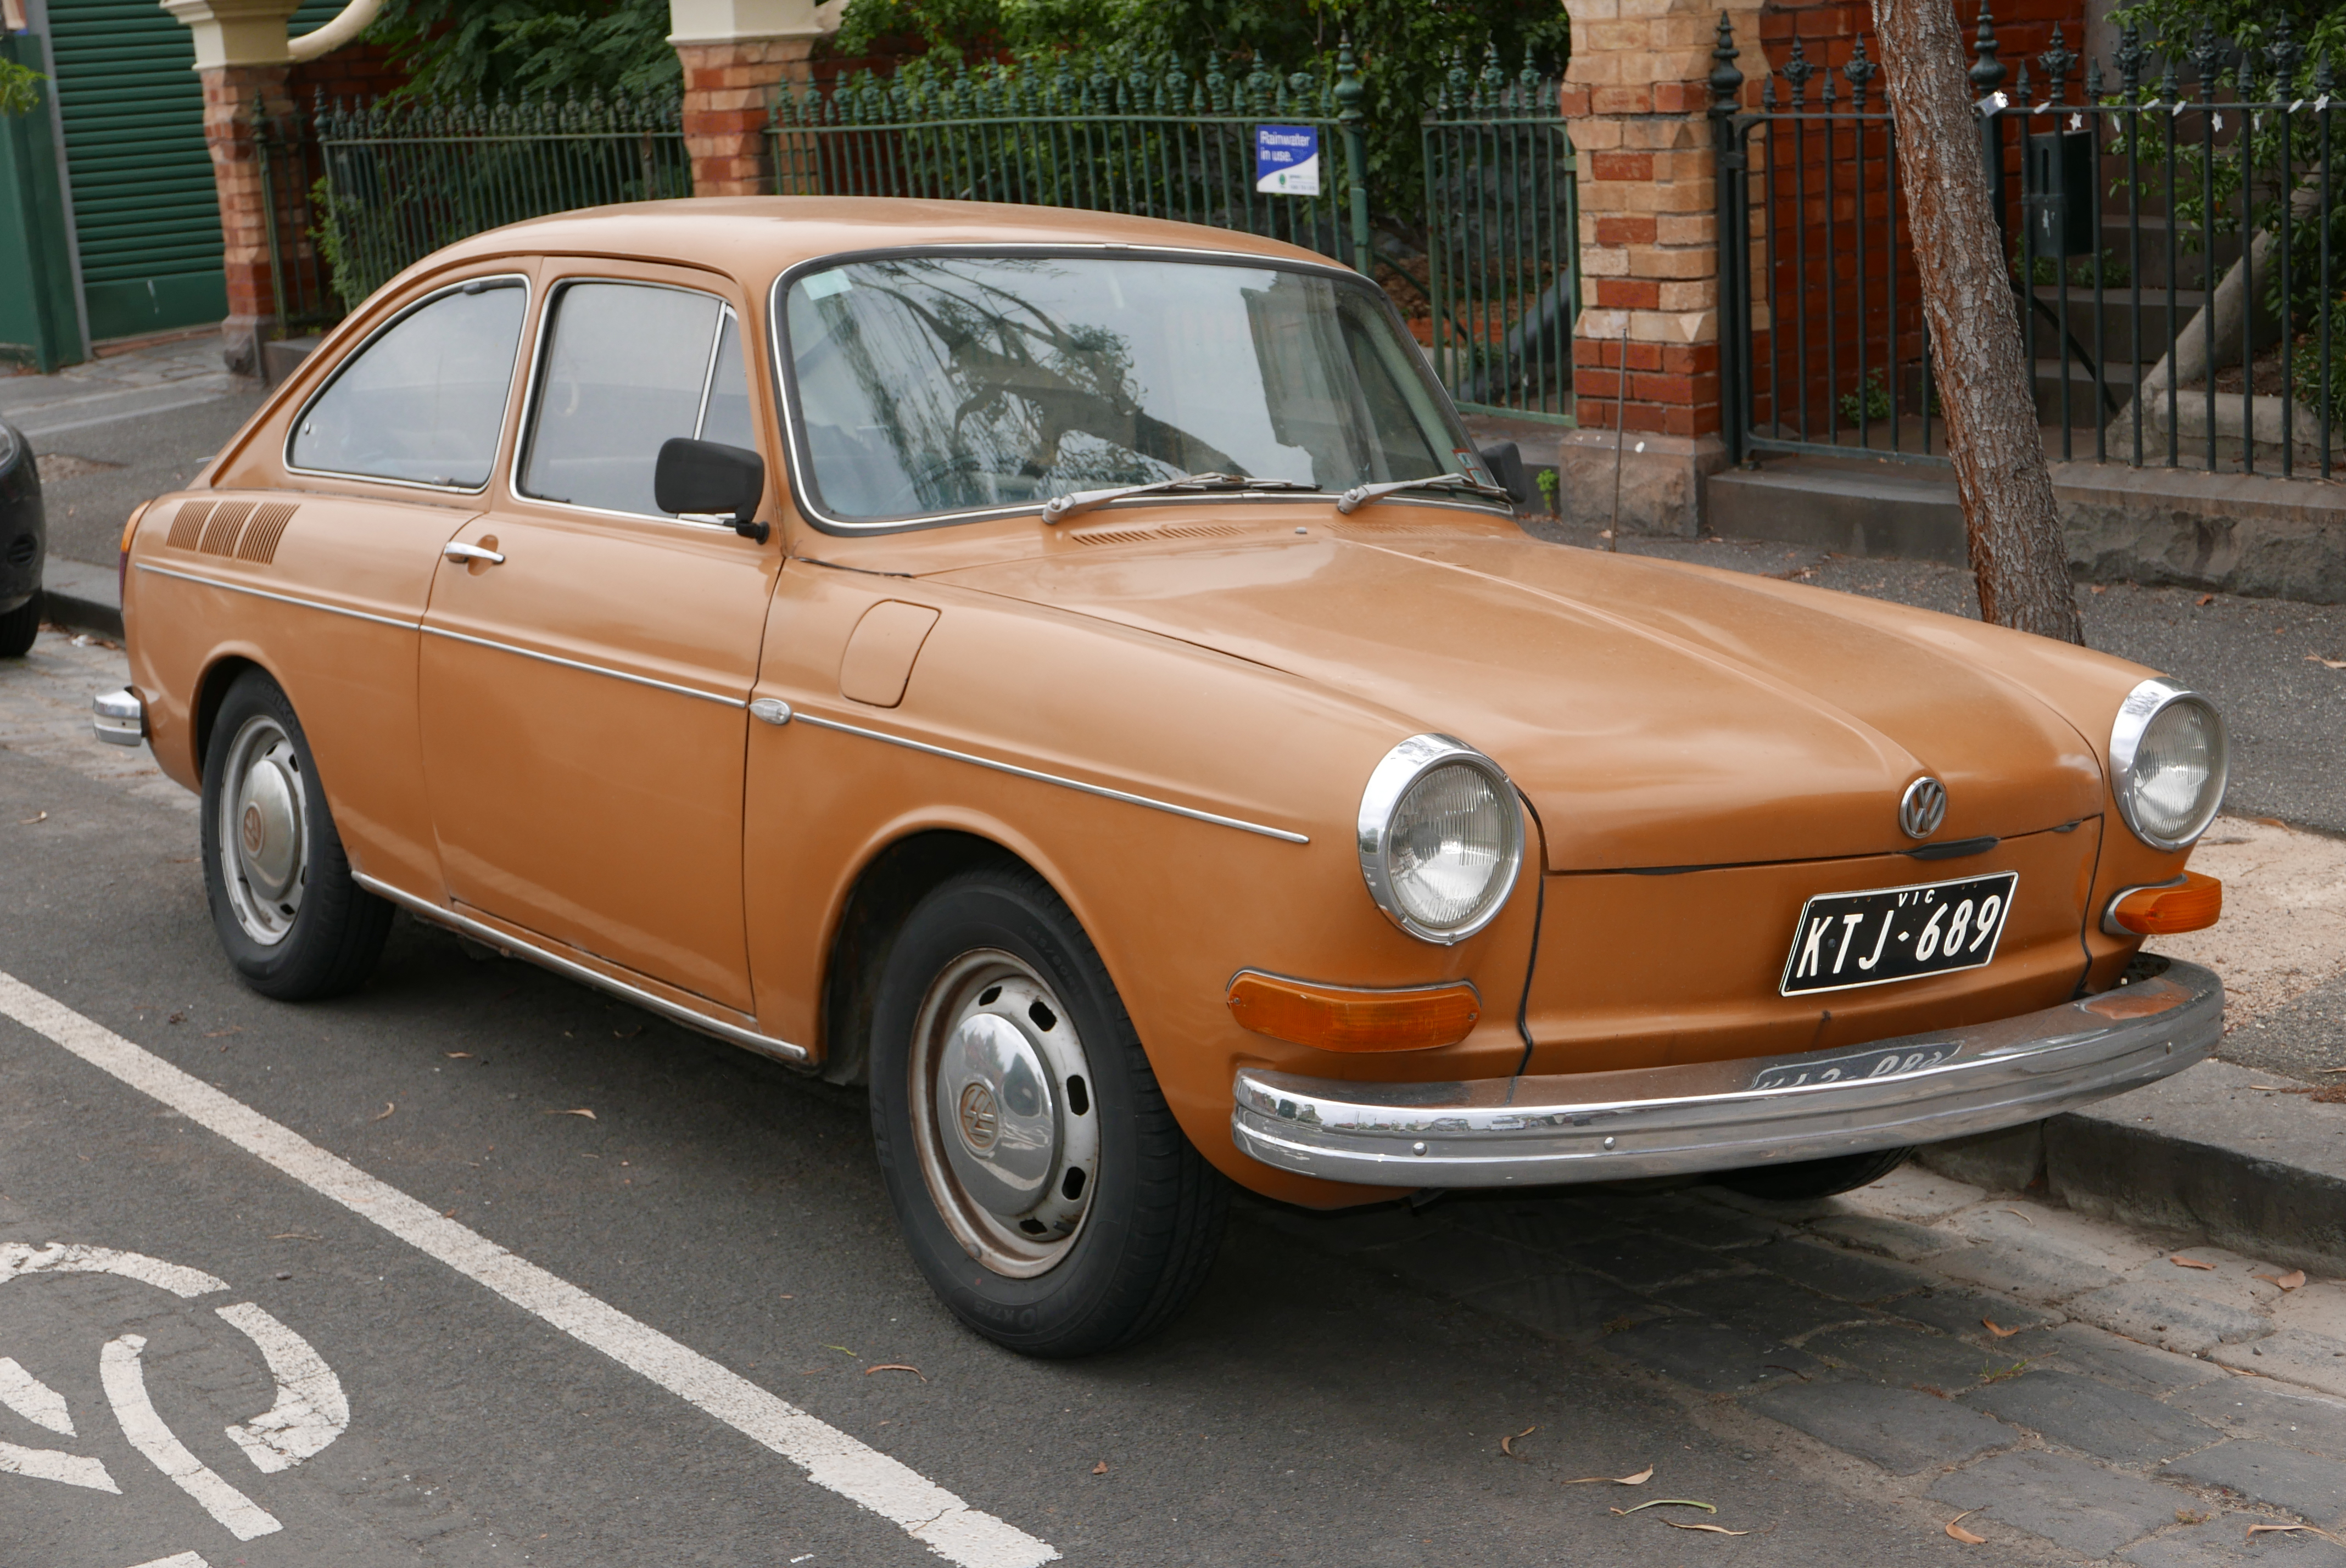
\includegraphics[width=.9\linewidth]{images/volkswagen_t3.jpg}
  \caption{Volkswagen Tipo III, modelo de inyección de 1969 -- de OSX - Trabajo propio \cite{VolkswagenTipo2021}.}
  \label{fig:volkswagen_t3}
\end{figure}

Pese a que supusieron un gran avance, estos primeros sistemas de
diagnóstico daban una información muy valiosa pero limitada, ya que muchos
diagnósticos seguirían siendo mediante los sentidos y las sensaciones
que le transmitiese el vehículo al mecánico. No fue hasta 1980 en donde
se implementó de forma estándar en los vehículos de \textit{General Motors}
el \ac{ALDL}, un lector de errores del coche que funcionó inicialmente a
160 baudios. Años más tarde, el sistema se refinaría usando el estándar
\ac{UART} \textit{half--duplex}, es decir, transmisión en los dos sentidos pero
no de forma simultánea (figura \ref{fig:aldl}). La principal motivación de incluir estos sistemas no fue
otra sino intentar reducir la contaminación de los vehículos teniendo
acceso a esta información \cite{SistemaOBD2Historia}.

\begin{figure}[H]
  \centering
  \includegraphics[width=.75\linewidth]{images/aldl.jpg}
  \caption{Conector \ac{ALDL}, creado por \textit{General Motors} antes de
  estandarizar OBD-II \cite{ReferenceManualChapter}.}
  \label{fig:aldl}
\end{figure}

No es hasta 1979 en que la \ac{SAE} recomienda crear un conector de
diagnóstico estandarizado en el mercado así como un conjunto de señales
de prueba. Finalmente, en 1991 la \ac{CARB} require que todos sus
vehículos tengan lo que sería el \ac{OBD}-I. Esta primera versión informaría
al conductor de un mal funcionamiento de alguno de los elementos del
vehículo mediante un \ac{MIL}, un indicador luminoso de fallos. Sin
embargo, solo se monitorizaban ciertos componentes relacionados con las
emisiones y no estaban calibrados \cite{SistemaOBD2Historia}.

Por ende, impulsado por las alertas \textit{smog} y por una fuerte regulación, en 1994
la \ac{CARB} obligó a todos los vehículos fabricados y vendidos a partir de 1996 incluir
el \ac{OBD}-II. Esto supuso un gran impulso en los mecanismos de monitorización de los
vehículos ya que además se estandarizó tanto el conector como los protocolos recomendados
por la \ac{SAE}. Tiempo más tarde, el Gobierno de los Estados Unidos aplicó la misma
medida a todos los vehículos del país \cite{SistemaOBD2Historia}.

Esta medida llegaría a Europa en 1998, según la Directiva 98/69EG, que obligaba a
todos los vehículos europeos a incluir dicho conector. Específicamente, los
automóviles de gasolina debían empezar a equiparlo en los modelos del año 2000; en el año 2003
para vehículos diésel; y en el año 2005 para camiones \cite{SistemaOBD2Historia}.

\subsection*{OBD--II}
\ac{OBD}--II es la segunda generación del sistema de diagnósticos de abordo, sucesor
de \ac{OBD}--I y su principal función es la de avisar al conductor cuando las
emisiones del vehículo son en torno a $1.5$ veces mayores de las diseñadas. A
diferencia de \ac{OBD}--I, \ac{OBD}--II también detecta fallos eléctricos, químicos
y mecánicos que puedan afectar al nivel de emisiones del vehículo (un caso típico
era un fallo químico del catalizador, indetectable por \ac{OBD}--I pero sí por la
segunda generación).

Este tipo de conector, al ser el primer estándar, cuenta con
múltiples interfaces que permiten conexiones mediante redes Wi-Fi, USB, Bluetooth,
etc. (cayendo pues en deshuso el protocolo de conexión por puerto serie -- RS232).
Esto se ha conseguido gracias al rápido avance de los sistemas embebidos, en donde
la combinación de \textit{software} y \textit{hardware} embebidos ha permitido que
cualquier usuario tenga acceso a este tipo de datos de forma relativamente simple
(actualmente, el conector más estandarizado es el controlador \texttt{ELM327} \cite{SistemaOBD2Historia},
figura \ref{fig:elm327}):

\begin{figure}[H]
  \centering
  \includegraphics[width=.7\linewidth]{images/obd-ii-elm327.jpg}
  \caption{Controlador \texttt{ELM327} que cuenta con antenas Wi-Fi y Bluetooth para un acceso remoto \cite{AmazonComElm327}.}
  \label{fig:elm327}
\end{figure}

El sistema verifica todos los sensores directamente involucrados con las emisiones
del vehículo, como por ejemplo la inyección de aire al motor. Cuando algún sensor detecta
un fallo, se activa el \ac{MIL} indicando el fallo que sucede (o una combinación
de indicadores para notificar la existencia de un fallo, sin especificar exactamente
cuál).

El vehículo que incorpora un conector \ac{OBD}--II almacena la información sobre el
fallo del vehículo para que el mecánico que deba revisar el automóvil disponga de todos
los datos posibles. Por otra parte, este estándar permite una comunicación directa
con el vehículo mediante el envío de órdenes según un \ac{PID}. Por defecto, hay
una serie de \ac{PID}s estándar que la gran mayoría de vehículos deben incluir\footnote{%
Se dice ``la mayoría de vehículos'' porque hay ciertos \ac{PID}s que dependen
directamente del tipo de vehículo (a combustión, eléctrico, \dots) o del combustible
utilizado -- un vehículo eléctrico no ofrece información sobre las \ac{RPM} al igual
que un vehículo diésel no ofrece información sobre las bujías.}, pero también
los fabricantes de vehículos incluyen una serie de \ac{PID}s propios (conocidos como
\textit{\ac{PID}s propietarios}) que ofrecen información adaptada a cada vehículo
en particular y que, en principio, son privados y cerrados al público en general.

En Europa se implantó el \ac{EOBD}, la variación europea del estándar \ac{OBD}--II
implantada en el año 2000 en general. Si bien en apariencia es semejante al \ac{OBD}--II,
las diferencias radican en el \textit{software}. Por ejemplo, el estándar europeo
no monitoriza las evaporaciones del depósito de combustible; sin embargo, es más
sofisticado ya que usa ``mapas'' en las entradas de los sensores que obligan a que el
sensor se calibre empíricamente al sistema según las condiciones de operación del
motor (lo cual se traduce en que los sensores son mucho mejores pero más caros)
\cite{SistemaOBD2Historia}. Otra característica innovadora es que el sistema
europeo registra cuántos kilómetros se han recorrido desde que ha aparecido un
defecto \cite{EOBDOBD2}.

Finalmente, pero no menos importante, Japón tiene también su propio estándar denominado
\ac{JOBD}.

\subsection*{OBD--III}
El \ac{OBD}--III se espera que sea la siguiente versión del sistema que ya implementan
los coches actualmente. La principal diferencia con respecto a la versión anterior
será que el vehículo estará conectado de forma continua y emitiendo datos referentes
a las emisiones. De esta forma, se puede saber casi en el momento acerca de modificaciones
ilegales, un aumento en la contaminación del coche (signo de deterioro) y demás. No se
espera igualmente que sea un salto cualitativo ya que se sigue buscando que sea
altamente compatible con las herramientas que ya existen. Actualmente, se están
realizando pruebas en EE.UU. pero no hay cerrada ninguna fecha de estandarización
oficial por parte de los distintos continentes.

\subsection{Herramientas de monitorización y control del automóvil}
Pese al tiempo que lleva \ac{OBD}--II disponible, las herramientas existentes para
la actuación sobre un vehículo son relativamente escasas. La mayoría de modelos
presentes hoy en día en el mercado se basan directa o indirectamente en el
\texttt{ELM327}, un dispositivo de diagnóstico \ac{OBD} que cuenta con conexión
WiFi, Bluetooth y serie para la lectura local.

Por lo general, las herramientas que hay se utilizan por mecánicos o fanáticos del
sector para acceder a la información del estado del vehículo y ver los errores que
pudiera tener. Sin embargo, tras una breve documentación sobre el tema, la mayoría
de los casos buscaban directamente monitorizar en el momento el estado
del vehículo para obtener información relativa a los consumos, contaminación,
etc.

Por ejemplo, en el trabajo de Rimpas \textit{et al.} \cite{rimpasOBDIISensorDiagnostics2020}, se utiliza
un sensor \texttt{ELM327} para verificar que la información proporcionada por
el puerto del vehículo y la presentada por la telemetría presente en el mismo
(velocímetro y tacómetro) son coherentes entre sí (previa adaptación de los
valores en \textit{bytes} presentados por el conector a valores legibles). En
dicha investigación se llega a la conclusión de que el conector \ac{OBD}--II obtiene
valores fiables y consistentes tanto con los mostrados por el propio vehículo
como los proporcionados por el fabricante.

Otro tipo de investigaciones llevadas a cabo gracias a la presencia de este conector
en los automóviles es la de la caracterización de conductores y hábitos de conducción
según la telemetría reportada por el vehículo. En el estudio realizado por
Galih Hermawan y Emir Husni \cite{hermawanAcquisitionModelingEvaluating2020} se
estudia la combinación de la lectura de los sensores mediante el \ac{OBD}--II con
vehículos que presentan el sistema \ac{ADAS}.
El estudio busca identificar hábitos de conducción según la lectura de los diversos
sensores que hay en el sistema. También persigue detectar quién es el conductor que
está llevando el vehículo actualmente. En el estudio, el uso de \ac{OBD}--II junto
con los algoritmos de los \textit{k--Nearest Neighbor} (k--NN) y \textit{Naive Bayes}
consiguieron una precisión en la identificación del 100\% (
para un conjunto de datos de 10 conductores).
Por otra parte, el uso de inteligencia artificial junto con técnicas de \textit{clustering}
permitieron identificar comportamientos de los conductores al volante y relacionarlo
además con situaciones de riesgo y peligro. Además, se ha aplicado a otras características
también interesantes como detectar el tipo de calzada, predecir el tiempo de viaje,
analizar el consumo del vehículo y demás. El esquema seguido en la investigación es el
que se presenta en la figura \ref{fig:investigation-scheme}:

\begin{figure}[H]
  \centering
  \includegraphics[width=.7\linewidth]{images/general-scheme-investigation.png}
  \caption{Esquema seguido para determinar los hábitos de conducción usando el \ac{OBD}--II \cite{hermawanAcquisitionModelingEvaluating2020}.}
  \label{fig:investigation-scheme}
\end{figure}

Por último, uno de los tipos de investigación bastante interesante realizada en los
últimos años es la de la generación de perfiles de conducción y de consumo. En el
artículo realizado por Ameen \textit{et al.} \cite{husseinaliameenDrivingBehaviourIdentification2021}
se define un sistema de clasificación del comportamiento del conductor al volante
(que es además el que se propone usar en este proyecto) el cual combina los datos
recibidos por el \ac{OBD}--II y del \ac{GPS} (figura \ref{fig:driving-behaviour}):

\begin{figure}[H]
  \centering
  \includegraphics[width=.7\linewidth]{images/driving-behaviour-workflow.png}
  \caption{Flujo de análisis para determinar el comportamiento al volante de un conductor \cite{husseinaliameenDrivingBehaviourIdentification2021}.}
  \label{fig:driving-behaviour}
\end{figure}

Al final, el estudio concluía con los siguientes perfiles de conducción:

\begin{itemize}
  \item \textbf{Peligroso}, para una aceleración en general superior a $7\ \nicefrac{m}{s^2}$.
  \item \textbf{Agresivo}, para una aceleración entre $\left[4\ \nicefrac{m}{s^2}, 7\ \nicefrac{m}{s^2}\right)$.
  \item \textbf{Normal}, para una aceleración entre $\left[2\ \nicefrac{m}{s^2}, 4 \nicefrac{m}{s^2}\right)$.
  \item \textbf{Seguro}, para una aceleración entre $\left[0\ \nicefrac{m}{s^2}, 2\ \nicefrac{m}{s^2}\right)$.
\end{itemize}

\section{Objetivos del desarrollo del proyecto}\label{sec:objectives}
Como se ha podido apreciar, existen multitud de aplicaciones relacionadas directa
o indirectamente con el \ac{OBD}--II, en parte por la longevidad del conector
en el mercado.

Sin embargo, todas o la gran mayoría de aplicaciones están destinadas a los profesionales
del sector, e incluso se ha aprovechado este conector para dificultar el acceso a
los datos del vehículo, habiendo de ir a un taller oficial para que puedan hacer
las reparaciones pertinentes.

Por otra parte, el parque de vehículos español es cada año más viejo debido a
diversos factores que no se van a analizar en este trabajo. Esto implica que cada
año más y más vehículos pierden el soporte por parte del fabricante y se vuelven
cada vez más costosos y complejos de mantener.

Para los no eruditos, el mundo del automóvil es el gran desconocido en donde una
serie de personas cualificadas se encargan del mantenimiento y correcto funcionamiento
del mecanismo que nos transporta por el mundo. Si bien es cierto que es necesaria
esta figura, hay una serie de buenas prácticas y actuaciones que pueden prevenir
tener que ir al mecánico de forma recurrente. Solo hace falta acceso a la información
de manera accesible.

Es por esto que nace \ac{VIMS}, un proyecto que pretende desarrollar un sistema completo
que consta de varias partes: un dispositivo embebido, un servidor y el usuario en sí
(figura \ref{fig:general-scheme}):

\begin{figure}[H]
  \centering
  \includegraphics[width=\linewidth]{images/general-scheme.png}
  \caption{Esquema general que modela el modo de funcionamiento del sistema.}
  \label{fig:general-scheme}
\end{figure}

La idea fundamental detrás de este proyecto es la de devolverle a los usuarios
el control sobre su vehículo, ser conscientes de cómo funciona o, al menos, entender
mejor qué pueden hacer para mejorar tanto su estilo de conducción como la seguridad
al volante. De esta forma, con el dispositivo se espera también prevenir riesgos
ya que los propietarios y usuarios de los vehículos estarán informados en todo
momento de qué error pueda tener.

Como se prevé que este dispositivo sea utilizado por una gran variedad de usuarios
es crucial que sea accesible en términos de sencillez de manejo, entendimiento y
uso: evitar datos excesivamente técnicos, presentar la información más relevante
primero, etc.

Para ello, se hará uso de plataformas en la nube para gestionar, almacenar y presentar
la información al usuario y se contará con una aplicación móvil que permita un
fácil acceso a los datos del vehículo, tanto históricos como generados en el momento.

Al igual que otros trabajos previamente realizados, el proyecto se realiza sobre
las filosofías del código libre y del \textit{hardware} libre, que se traduce en
que todos los recursos (tanto físicos como \textit{software}) estarán disponibles
enteramente para cualquier persona interesada en ver cómo funciona, replicar el
proyecto por su cuenta y contar con plena potestad para mejorarlo, redistribuirlo
y trabajar con él (siempre bajo un prisma de reconocimiento al autor original
del trabajo regido por \textit{copyright}). Para ello, se ha decidido hacer uso
de la licencia MIT\footnote{Se pueden obtener más detalles sobre la licencia MIT
en la siguiente URL: \url{https://choosealicense.com/licenses/mit/}}.

\section{Metodología}\label{sec:methodology}
El proyecto que se pretende desarrollar es un proyecto de ingeniería. Esto se
traduce en que la metodología y la forma de trabajo son pilares fundamentales
en el desarrollo del mismo.

El primer paso realizado fue el de recopilar recursos e información de qué
necesitaban específicamente los usuarios. Para ello, se elaboró un cuestionario
en donde de forma general se preguntaba a conductores y no conductores qué querrían
tener en su vehículo. Los primeros sirvieron como fuente de información principal,
debido a sus características \textit{per se}; los segundos para aumentar la entropía
de los datos obtenidos y usando sus respuestas como grupo de control para validar la
de los primeros. El primer análisis realizado se detalla
en la sección \ref{ssec:user-req}, de la especificación de requisitos. Posteriormente,
en el punto \ref{sec:merch} se analiza en mayor profundidad los datos obtenidos
y se extraerán conclusiones.

A continuación, se realizó un estudio sobre qué plataformas y dispositivos están
accesibles de forma global para la generación y transmisión de datos. Esta fase
se centró principalmente en ``descubrir'' variantes del modelo ESP32 que incluyesen
ciertas antenas para permitir una mayor conectividad. Tras valorar diversas opciones,
se decidió usar el LILYGO T-SIM7000G ESP32 que incluye soporte de forma nativa para
tarjetas microSD, antena \ac{LTE}, alimentación externa por batería, antena \ac{GPS}, WiFi y
Bluetooth.

Una vez se decidió que dispositivo físico se iba a utilizar, se comenzó con el desarrollo
de los distintos diagramas que modelan el sistema, tanto lógicos como de diseño. Esta
parte fue crucial para asentar las bases de lo que será el proyecto y ha permitido seguir
el avance del mismo.

Por último, se realizó el serigrafiado de la placa y se comenzó la implementación
física de los diseños realizados. Por diversos contratiempos que han surgido, el proyecto
se ha planteado finalmente como proyecto de especificación y diseño, con una batería
de ensayos específicos reales que facilitarán la construcción que se va a realizar
posteriormente.


%% Product description
\chapter{Estructura del proyecto}\label{chap:structure}
El desarrollo del sistema \ac{VIMS} es un proceso multidisciplinar en el que se deben
desarrollar varias áreas de conocimiento. Este proyecto se ha postulado como
un desarrollo integral de ingeniería y es por eso por lo que está dividido en
varios bloques que conforman un factor clave en el desarrollo del mismo.

Estas secciones están bien diferenciadas y se conforman de: un estudio de mercado y de
las características de los usuarios, un estudio matemático asociado a la lectura de
valores y adecuación del \textit{hardware}, el proceso de diseño \textit{hardware}
en sí, el diseño \textit{software} del sistema y el análisis de planificación del mismo.

\begin{itemize}
  \item El estudio de mercado pretende averiguar y formalizar las necesidades de los
  conductores y usuarios de la vía. Es la primera aproximación y facilita la
  delimitación del producto y, sobre todo, ofrecerle al usuario final algo de utilidad
  y que pueda necesitar.
  \item El estudio matemático se encarga de investigar la ``traducción'' de los
  valores recibidos por el vehículo (según los datos asociados al estudio de mercado
  realizado con anterioridad).
  \item El diseño \textit{software} modela principalmente cómo se va a estructurar
  el sistema y cómo debe comportarse ante los distintos eventos que puede recibir.
  Esta fase conlleva realizar diagramas lógicos y de diseño del sistema en su conjunto.
  \item El diseño \textit{hardware} conlleva tanto el estudio de los componentes del
  sistema así como de las restricciones físicas del mismo.
  \item El análisis de planificabilidad complementa el diseño \textit{software}
  y estudia si el sistema es planificable. En los requisitos no se define \ac{VIMS}
  como un sistema en tiempo real, pero la cantidad de componentes que contiene y las
  acciones que tiene que realizar requieren del uso de subrutinas y de una planificación
  previa para asegurar un correcto funcionamiento del mismo.
\end{itemize}

Es importante detallar que pese a que el sistema se compone de varios componentes,
son dos los principales que lo caracterizan:

\begin{enumerate}
  \item La placa, \ac{VIMS}, que va embebida en los vehículos del sistema. Se encarga
  de toda la lectura, adaptación y emisión de datos. Además, cuenta con soporte para
  poder realizar una transmisión de la información a un dispositivo asociado mediante
  redes \ac{PAN}.
  \item El servidor \textit{cloud}, el ``cerebro'' encargado de recibir las tramas,
  los datos y la información relativa a las placas \ac{VIMS}, los dispositivos de
  usuario y demás componentes. Además, tiene la responsabilidad de ofrecer a los
  usuarios una \ac{GUI}, generar información relevante a partir de los datos (como
  estadísticas), gestionar las suscripciones y enviar periódicamente la información
  al usuario.
\end{enumerate}

\section{Estudio de mercado}\label{sec:merch}
Para el desarrollo de este proyecto, se hizo un estudio de mercado tanto de los
consumidores como de sus características, además de una evaluación exhaustiva
de qué les gustaría tener en su vehículo.

Este proyecto pretende en un futuro salir a mercado y suplir características que los
usuarios echan en falta en sus correspondientes medios de transporte. Como en principio
funciona con cualquier vehículo que cuente con \ac{OBD}--II, las respuestas no se han
limitado a aquellos conductores que condujesen turismos sino cualquier tipo de
automóvil: motocicleta, camión, etc.

Es importante destacar que el estudio tiene varios sesgos que han restringido
y delimitado las respuestas que se han registrado:

\begin{enumerate}
  \item Se ha realizado un cuestionario usando Google Forms, una plataforma de Google
        que permite preparar una serie de preguntas y respuestas y aplicar ciertos
        filtros sobre ellas. Por ejemplo, para aquellos que dijeron ser conductores,
        se hicieron preguntas diferentes frente a quienes no lo fueran.

        Esto permite obtener datos más fidedignos y acotados según la población que
        respondiera. Sin embargo, tiene una limitación implícita: restringe el acceso
        a aquellos con conocimientos ``suficientes'' acerca de la plataforma. Pese
        a que el producto pretende ser lo más accesible posible, no hy que olvidar
        que este tipo de tecnologías permanecen desconocidas para una gran parte
        de la población con escasos conocimientos acerca de Internet o de las
        nuevas tecnologías. Se comentará más adelante, pero esto se ve reflejado
        principalmente en la edad media de quienes respondieron el cuestionario.

        Por otra parte, al ser un cuestionario aparece otra limitación implícita
        y es la validación y verificación de las respuestas.
\end{enumerate}

\section{Estudio matemático}\label{sec:maths}
El estudio matemático va muy ligado al punto anterior (\ref{sec:merch}) ya que se
analizan los parámetros de \ac{OBD}--II y su ecuación matemática para obtener un
valor en $\mathbb{R}$ entendible por las personas.

Antes de dar paso a las ecuaciones en sí, es importante entender cómo funciona
el conector \ac{OBD}--II en esta situación. Los datos enviados y recibidos por
el coche están siempre codificados en un valor binario, recogido en un vector
de cuatro elementos en donde cada elemento tiene un \textit{byte} de tamaño. De
esta forma, se define al valor obtenido tras leer el conector \ac{OBD}--II como:

\begin{table}[H]
  \centering
  \resizebox{\textwidth}{!}{\begin{tabular}{|c|c|c|c|c|c|c|c|c|c|c|c|c|c|c|c|c|c|c|c|c|c|c|c|c|c|c|c|c|c|c|c|}
      \hline
      \multicolumn{8}{|c|}{$A$} & \multicolumn{8}{|c|}{$B$} & \multicolumn{8}{|c|}{$C$} & \multicolumn{8}{|c|}{$D$}                                                                                                                                                                                                                                 \\
      \hline
      $A_7$                     & $A_6$                     & $A_5$                     & $A_4$                     & $A_3$ & $A_2$ & $A_1$ & $A_0$ & $B_7$ & $B_6$ & $B_5$ & $B_4$ & $B_3$ & $B_2$ & $B_1$ & $B_0$ & $C_7$ & $C_6$ & $C_5$ & $C_4$ & $C_3$ & $C_2$ & $C_1$ & $C_0$ & $D_7$ & $D_6$ & $D_5$ & $D_4$ & $D_3$ & $D_2$ & $D_1$ & $D_0$ \\
      \hline
    \end{tabular}}
  \caption{Vector de \textit{bytes} que representa los datos recibidos del conector \ac{OBD}--II \cite{OBDIIPIDs2021}.}
  \label{tab:byte-array}
\end{table}

De esta forma, cuando se escribe $A_4$ se hace referencia al cuarto bit
del vector $A$. Los bits están ordenados según \ac{MSB}, de forma que
$A_7$ es el bit más significativo y $A_0$ el menor.

Los datos se obtienen del \ac{OBD}--II utilizando un lenguaje estándar llamado
\ac{PID}. El \ac{PID} se codifica como un número entero de 16 bits en donde los 8
primeros bits identifican el servicio/modo y los 8 restantes la operación a realizar.
Actualmente, están registrados los siguientes modos de funcionamiento (tabla
\ref{tab:pids-mode}):

\begin{table}[H]
  \centering
  \begin{tabularx}{\textwidth}{ | c | X | }
    \hline
    \textbf{Modo (hex)} & \textbf{Descripción}                                                                       \\
    \hline
    \texttt{01}         & Muestra los datos actuales del vehículo                                                    \\
    \hline
    \texttt{02}         & Muestra los datos almacenados del cuadro del vehículo                                      \\
    \hline
    \texttt{03}         & Muestra los códigos \ac{DTC}                                                               \\
    \hline
    \texttt{04}         & Elimina los códigos \ac{DTC} almacenados                                                   \\
    \hline
    \texttt{05}         & Resultados del test del sensor de oxígeno (sin \ac{CAN})                                   \\
    \hline
    \texttt{06}         & Resultados del test del sensor de oxígeno (con \ac{CAN})                                   \\
    \hline
    \texttt{07}         & Muestra los códigos \ac{DTC} pendientes (eliminados durante el último ciclo de conducción) \\
    \hline
    \texttt{08}         & Operaciones de control sobre los componentes del sistema                                   \\
    \hline
    \texttt{09}         & Petición de información sobre el vehículo                                                  \\
    \hline
    \texttt{0A}         & Códigos \ac{DTC} eliminados                                                                \\
    \hline
  \end{tabularx}
  \caption{Lista de modos de funcionamiento del estándar \ac{OBD}--II \cite{OBDIIPIDs2021}.}
  \label{tab:pids-mode}
\end{table}

Es importante destacar que no todos los fabricantes tienen por qué soportar todos
los modos, y que además ciertos fabricantes pueden definir sus modos propios por encima
del valor \texttt{09}.

Todos los modos definidos anteriormente tienen un conjunto de órdenes de soporte
en donde el sistema indica qué \ac{PID}s están soportados y cuáles no, por cada 32
\ac{PID}s. Por ejemplo, enviar la orden \texttt{0x0100} (\textit{modo 1, PID 0})
devolverá un valor que representará si los siguientes 32 \ac{PID}s están soportados.
Si el valor fuese, por ejemplo, \texttt{BE1FA813} se tendría que:

\begin{table}[H]
  \centering
  \resizebox{\textwidth}{!}{\begin{tabular}{ | c | c | c | c | c | c | c | c | c | c | c | c | c | c | c | c | c | c | c | c | c | c | c | c | c | c | c | c | c | c | c | c | c | }
      \hline
      \textbf{Hexadecimal} & \multicolumn{4}{|c|}{\texttt{B}} & \multicolumn{4}{|c|}{\texttt{E}} & \multicolumn{4}{|c|}{\texttt{1}} & \multicolumn{4}{|c|}{\texttt{F}} & \multicolumn{4}{|c|}{\texttt{A}} & \multicolumn{4}{|c|}{\texttt{8}} & \multicolumn{4}{|c|}{\texttt{1}} & \multicolumn{4}{|c|}{\texttt{3}}                                                                                                                                                                                                                                                                                                                                                 \\
      \hline
      \textbf{Binario}     & \texttt{1}                       & \texttt{0}                       & \texttt{1}                       & \texttt{1}                       & \texttt{1}                       & \texttt{1}                       & \texttt{1}                       & \texttt{0}                       & \texttt{0}  & \texttt{0}  & \texttt{0}  & \texttt{1}  & \texttt{1}  & \texttt{1}  & \texttt{1}  & \texttt{1}  & \texttt{1}  & \texttt{0}  & \texttt{1}  & \texttt{0}  & \texttt{1}  & \texttt{0}  & \texttt{0}  & \texttt{0}  & \texttt{0}  & \texttt{0}  & \texttt{0}  & \texttt{1}  & \texttt{0}  & \texttt{0}  & \texttt{1}  & \texttt{1}  \\
      \hline
      \textbf{¿Soportado?} & \done                            & \wontfix                         & \done                            & \done                            & \done                            & \done                            & \done                            & \wontfix                         & \wontfix    & \wontfix    & \wontfix    & \done       & \done       & \done       & \done       & \done       & \done       & \wontfix    & \done       & \wontfix    & \done       & \wontfix    & \wontfix    & \wontfix    & \wontfix    & \wontfix    & \wontfix    & \done       & \wontfix    & \wontfix    & \done       & \done       \\
      \hline
      \textbf{PID}         & \texttt{01}                      & \texttt{02}                      & \texttt{03}                      & \texttt{04}                      & \texttt{05}                      & \texttt{06}                      & \texttt{07}                      & \texttt{08}                      & \texttt{09} & \texttt{0A} & \texttt{0B} & \texttt{0C} & \texttt{0D} & \texttt{0E} & \texttt{0F} & \texttt{10} & \texttt{11} & \texttt{12} & \texttt{13} & \texttt{14} & \texttt{15} & \texttt{16} & \texttt{17} & \texttt{18} & \texttt{19} & \texttt{1A} & \texttt{1B} & \texttt{1C} & \texttt{1D} & \texttt{1E} & \texttt{1F} & \texttt{20} \\
      \hline
    \end{tabular}}
  \caption{Obtención de los \ac{PID}s soportados según el modo \cite{OBDIIPIDs2021}.}
  \label{tab:supported-pids}
\end{table}

A continuación, se dejan un conjunto de \ac{PID}s que se van a implementar en el
proyecto así como el código de acceso a ellos y la ecuación que permite obtener el
valor real.

\subsection*{Modo \texttt{01}}
Este modo permite acceder a la información en tiempo real del vehículo, según se
está en marcha. Los datos a los que se accede son:

\begin{table}[H]
  \centering
  \begin{tabularx}{\textwidth}{|c|X|}
    \hline
    \textbf{PID (hex)}       & \texttt{04}                    \\
    \hline
    \textbf{Bytes devueltos} & $1$                            \\
    \hline
    \textbf{Descripción}     & Carga del motor, en porcentaje \\
    \hline
    \textbf{Valor mínimo}    & $0\%$                          \\
    \hline
    \textbf{Valor máximo}    & $100\%$                        \\
    \hline
    \textbf{Fórmula}         &                                %
    \begin{equation*}
      \frac{A}{2.55}
    \end{equation*}                                 \\
    \hline
  \end{tabularx}
  \caption{\ac{PID} \texttt{04} -- carga del motor, en $\%$.}
\end{table}

\begin{table}[H]
  \centering
  \begin{tabularx}{\textwidth}{|c|X|}
    \hline
    \textbf{PID (hex)}       & \texttt{05}                    \\
    \hline
    \textbf{Bytes devueltos} & $1$                            \\
    \hline
    \textbf{Descripción}     & Temperatura del refrigerante del motor \\
    \hline
    \textbf{Valor mínimo}    & $-40~\tccentigrade$                          \\
    \hline
    \textbf{Valor máximo}    & $215~\tccentigrade$                        \\
    \hline
    \textbf{Fórmula}         &                                %
    \begin{equation*}
      A - 40
    \end{equation*}                                 \\
    \hline
  \end{tabularx}
  \caption{\ac{PID} \texttt{05} -- temperatura del refrigerante del motor, en $\tccentigrade$.}
\end{table}

\begin{table}[H]
  \centering
  \begin{tabularx}{\textwidth}{|c|X|}
    \hline
    \textbf{PID (hex)}       & \texttt{0C}                    \\
    \hline
    \textbf{Bytes devueltos} & $2$                            \\
    \hline
    \textbf{Descripción}     & Velocidad del motor \\
    \hline
    \textbf{Valor mínimo}    & $0~RPM$                          \\
    \hline
    \textbf{Valor máximo}    & $16383.75~RPM$                        \\
    \hline
    \textbf{Fórmula}         &                                %
    \begin{equation*}
      \frac{256A + B}{4}
    \end{equation*}                                 \\
    \hline
  \end{tabularx}
  \caption{\ac{PID} \texttt{0C} -- velocidad del motor, en $RPM$.}
\end{table}

\begin{table}[H]
  \centering
  \begin{tabularx}{\textwidth}{|c|X|}
    \hline
    \textbf{PID (hex)}       & \texttt{0D}                    \\
    \hline
    \textbf{Bytes devueltos} & $1$                            \\
    \hline
    \textbf{Descripción}     & Velocidad del vehículo \\
    \hline
    \textbf{Valor mínimo}    & $0~\nicefrac{km}{h}$                          \\
    \hline
    \textbf{Valor máximo}    & $255~\nicefrac{km}{h}$                        \\
    \hline
    \textbf{Fórmula}         &                                %
    \begin{equation*}
      A
    \end{equation*}                                 \\
    \hline
  \end{tabularx}
  \caption{\ac{PID} \texttt{0D} -- velocidad del vehículo, en $\nicefrac{km}{h}$.}
\end{table}

\begin{table}[H]
  \centering
  \begin{tabularx}{\textwidth}{|c|X|}
    \hline
    \textbf{PID (hex)}       & \texttt{11}                    \\
    \hline
    \textbf{Bytes devueltos} & $1$                            \\
    \hline
    \textbf{Descripción}     & Posición del acelerador \\
    \hline
    \textbf{Valor mínimo}    & $0\%$                          \\
    \hline
    \textbf{Valor máximo}    & $100\%$                        \\
    \hline
    \textbf{Fórmula}         &                                %
    \begin{equation*}
      \frac{A}{2.55}
    \end{equation*}                                 \\
    \hline
  \end{tabularx}
  \caption{\ac{PID} \texttt{11} -- posición del acelerador, en $\%$.}
\end{table}

\begin{table}[H]
  \centering
  \begin{tabularx}{\textwidth}{|c|X|}
    \hline
    \textbf{PID (hex)}       & \texttt{2F}                    \\
    \hline
    \textbf{Bytes devueltos} & $1$                            \\
    \hline
    \textbf{Descripción}     & Nivel del tanque del combustible \\
    \hline
    \textbf{Valor mínimo}    & $0\%$                          \\
    \hline
    \textbf{Valor máximo}    & $100\%$                        \\
    \hline
    \textbf{Fórmula}         &                                %
    \begin{equation*}
      \frac{A}{2.55}
    \end{equation*}                                 \\
    \hline
  \end{tabularx}
  \caption{\ac{PID} \texttt{2F} -- nivel del tanque del combustible, en $\%$.}
\end{table}

\begin{table}[H]
  \centering
  \begin{tabularx}{\textwidth}{|c|X|}
    \hline
    \textbf{PID (hex)}       & \texttt{46}                    \\
    \hline
    \textbf{Bytes devueltos} & $1$                            \\
    \hline
    \textbf{Descripción}     & Temperatura ambiente \\
    \hline
    \textbf{Valor mínimo}    & $-40~\tccentigrade$                          \\
    \hline
    \textbf{Valor máximo}    & $215~\tccentigrade$                        \\
    \hline
    \textbf{Fórmula}         &                                %
    \begin{equation*}
      A - 40
    \end{equation*}                                 \\
    \hline
  \end{tabularx}
  \caption{\ac{PID} \texttt{46} -- temperatura ambiente, en $\tccentigrade$.}
\end{table}

\begin{table}[H]
  \centering
  \begin{tabularx}{\textwidth}{|c|X|}
    \hline
    \textbf{PID (hex)}       & \texttt{5B}                    \\
    \hline
    \textbf{Bytes devueltos} & $1$                            \\
    \hline
    \textbf{Descripción}     & Tiempo restante de la batería híbrida \\
    \hline
    \textbf{Valor mínimo}    & $0\%$                          \\
    \hline
    \textbf{Valor máximo}    & $100\%$                        \\
    \hline
    \textbf{Fórmula}         &                                %
    \begin{equation*}
      \frac{A}{2.55}
    \end{equation*}                                 \\
    \hline
  \end{tabularx}
  \caption{\ac{PID} \texttt{5B} -- tiempo restante de la batería híbrida, en $\%$.}
\end{table}

\begin{table}[H]
  \centering
  \begin{tabularx}{\textwidth}{|c|X|}
    \hline
    \textbf{PID (hex)}       & \texttt{5C}                    \\
    \hline
    \textbf{Bytes devueltos} & $1$                            \\
    \hline
    \textbf{Descripción}     & Temperatura del aceite \\
    \hline
    \textbf{Valor mínimo}    & $-40~\tccentigrade$                          \\
    \hline
    \textbf{Valor máximo}    & $215~\tccentigrade$                        \\
    \hline
    \textbf{Fórmula}         &                                %
    \begin{equation*}
      A - 40
    \end{equation*}                                 \\
    \hline
  \end{tabularx}
  \caption{\ac{PID} \texttt{5C} -- temperatura del aceite, en $\tccentigrade$.}
\end{table}

\begin{table}[H]
  \centering
  \begin{tabularx}{\textwidth}{|c|X|}
    \hline
    \textbf{PID (hex)}       & \texttt{5E}                    \\
    \hline
    \textbf{Bytes devueltos} & $2$                            \\
    \hline
    \textbf{Descripción}     & Consumo actual del motor \\
    \hline
    \textbf{Valor mínimo}    & $0~\nicefrac{L}{h}$                          \\
    \hline
    \textbf{Valor máximo}    & $3212.75~\nicefrac{L}{h}$                        \\
    \hline
    \textbf{Fórmula}         &                                %
    \begin{equation*}
      \frac{256A + B}{20}
    \end{equation*}                                 \\
    \hline
  \end{tabularx}
  \caption{\ac{PID} \texttt{5E} -- consumo actual del motor, en $\nicefrac{L}{h}$.}
\end{table}

\begin{table}[H]
  \centering
  \begin{tabularx}{\textwidth}{|c|X|}
    \hline
    \textbf{PID (hex)}       & \texttt{61}                    \\
    \hline
    \textbf{Bytes devueltos} & $1$                            \\
    \hline
    \textbf{Descripción}     & Torque demandado por el conductor \\
    \hline
    \textbf{Valor mínimo}    & $-125\%$                          \\
    \hline
    \textbf{Valor máximo}    & $130\%$                        \\
    \hline
    \textbf{Fórmula}         &                                %
    \begin{equation*}
      A - 125
    \end{equation*}                                 \\
    \hline
  \end{tabularx}
  \caption{\ac{PID} \texttt{61} -- torque demandado por el conductor, en $\%$.}
\end{table}

\begin{table}[H]
  \centering
  \begin{tabularx}{\textwidth}{|c|X|}
    \hline
    \textbf{PID (hex)}       & \texttt{62}                    \\
    \hline
    \textbf{Bytes devueltos} & $1$                            \\
    \hline
    \textbf{Descripción}     & Torque actual del motor \\
    \hline
    \textbf{Valor mínimo}    & $-125\%$                          \\
    \hline
    \textbf{Valor máximo}    & $130\%$                        \\
    \hline
    \textbf{Fórmula}         &                                %
    \begin{equation*}
      A - 125
    \end{equation*}                                 \\
    \hline
  \end{tabularx}
  \caption{\ac{PID} \texttt{62} -- torque actual del motor, en $\%$.}
\end{table}

\begin{table}[H]
  \centering
  \begin{tabularx}{\textwidth}{|c|X|}
    \hline
    \textbf{PID (hex)}       & \texttt{63}                    \\
    \hline
    \textbf{Bytes devueltos} & $2$                            \\
    \hline
    \textbf{Descripción}     & Torque de referencia del motor \\
    \hline
    \textbf{Valor mínimo}    & $0~N \cdot M$                          \\
    \hline
    \textbf{Valor máximo}    & $65535~N \cdot M$                        \\
    \hline
    \textbf{Fórmula}         &                                %
    \begin{equation*}
      256A + B
    \end{equation*}                                 \\
    \hline
  \end{tabularx}
  \caption{\ac{PID} \texttt{63} -- torque de referencia del motor, en $N \cdot M$.}
\end{table}

\begin{table}[H]
  \centering
  \begin{tabularx}{\textwidth}{|c|X|}
    \hline
    \textbf{PID (hex)}       & \texttt{A4}                    \\
    \hline
    \textbf{Bytes devueltos} & $4$                            \\
    \hline
    \textbf{Descripción}     & Marcha actual del vehículo \\
    \hline
    \textbf{Valor mínimo}    & $0~\text{ratio}$                          \\
    \hline
    \textbf{Valor máximo}    & $65535~\text{ratio}$                        \\
    \hline
    \textbf{Fórmula}         &                                %
    \begin{equation*}
      \begin{aligned}
        A_1 &= 1 \Rightarrow \text{soportado} \\
        R &= \frac{256C + D}{1000}
      \end{aligned}
    \end{equation*}                                 \\
    \hline
  \end{tabularx}
  \caption{\ac{PID} \texttt{A4} -- marcha actual del vehículo, en ratio.}
\end{table}

\begin{table}[H]
  \centering
  \begin{tabularx}{\textwidth}{|c|X|}
    \hline
    \textbf{PID (hex)}       & \texttt{A6}                    \\
    \hline
    \textbf{Bytes devueltos} & $4$                            \\
    \hline
    \textbf{Descripción}     & Odómetro \\
    \hline
    \textbf{Valor mínimo}    & $0~km$                          \\
    \hline
    \textbf{Valor máximo}    & $429496729.5~km$                        \\
    \hline
    \textbf{Fórmula}         &                                %
    \begin{equation*}
      \frac{A\left(2^{24}\right) + B\left(2^{16}\right) + C\left(2^8\right) + D}{10}
    \end{equation*}                                 \\
    \hline
  \end{tabularx}
  \caption{\ac{PID} \texttt{A6} -- odómetro, en $km$.}
\end{table}

\section{Diseño \textit{software}}\label{sec:software}
El proyecto cuenta con una parte \textit{software} muy importante, ya que está
conformado por múltiples sistemas que deben cooperar entre sí. Por una parte,
el desarrollo del \textit{software} del proyecto aborda los siguientes aspectos:

\begin{itemize}
  \item Desarrollo de la aplicación embebida que irá en el dispositivo enganchado
        al coche en sí. En dicho dispositivo se programará, entre otros, la planificación
        del sistema según el análisis de planificabilidad llevado a cabo en el punto
        \ref{sec:rt-design}, la gestión de los datos y de la información y la transmisión
        al servidor remoto.
  \item Desarrollo de la infraestructura en la nube que alojará la lógica de almacenamiento de
        los datos y de la información generada a partir de ellos para los usuarios de
        dispositivos \ac{VIMS}.
  \item Desarrollo de la aplicación web que servirá de pasarela entre los usuarios
        y sus datos alojados en el servidor en la nube, mediante una interfaz de usuario
        que facilitará ciertas tareas de gestión y la observación de los datos.
  \item Desarrollo de la aplicación móvil que permitirá la conexión directa con la
        placa \ac{VIMS} para su configuración inicial y la visualización de la información
        en el momento.
\end{itemize}

El sistema sigue el prototipo de una arquitectura cliente--servidor, con uno o varios
clientes que se conectan a un servidor en la nube que realiza tareas de gestión de
la información, entre otros.

Uno de los requisitos principales de la aplicación (que se vio además en el estudio
del mercado) era que esta fuese accesible, simple y fácil de entender. Mediante la
definición de tanto la aplicación web como la aplicación móvil se pretende unificar
el acceso a la información de los usuarios y sus vehículos. Con ambas aplicaciones,
se busca que, de un vistazo, se tenga acceso a los últimos viajes, estadísticas,
perfiles de conducción y demás.

Además, la arquitectura del servidor permite generar notificaciones personalizadas
cuando sucedan ciertos eventos. Por ejemplo, se pueden enviar correos electrónicos
con información sobre el último viaje, cuánto ha durado el depósito de gasolina, fecha
recomendada para el siguiente mantenimiento, revisión del estado de los neumáticos,
etc. De esta manera, se pretende que el usuario no esté directamente pendiente del
estado mecánico de su vehículo sino que delegue esa tarea en el sistema \ac{VIMS}.

Por su lado, la programación del dispositivo \ac{VIMS} en sí es una parte crítica y
fundamental en el desarrollo del proyecto. El dispositivo va a estar en un entorno
no controlado con condiciones cambiantes, sobre todo en lo referente a las comunicaciones.
Es fundamental que \textit{software} del dispositivo embebido
sea resiliente y esté diseñado para soportar situaciones adversas en lo referente
a la transmisión de la información.

Esto se detalla más adelante en los requisitos, y algunas de las características que
se necesitan tener en el dispositivo en sí son el almacenamiento provisional de los
datos, la retransmisión de la información en caso de fallo, modos de bajo consumo
cuando el vehículo no está en marcha, etc.

\section{Diseño \textit{hardware}}\label{sec:hardware}
Los elementos \textit{hardware} hacen referencia directa al dispositivo \ac{VIMS}
que irá embebido en el vehículo y al resto de componentes que son necesarios para
un correcto funcionamiento del mismo. En esta sección también se incluye el
diseño 3D de la caja contenedora del dispositivo.

En términos generales, el \textit{hardware} en que se descompone el proyecto es:

\begin{itemize}
  \item Dispositivo controlador \ac{SoC} ESP32, que incluye de fábrica radios WiFi y Bluetooth.
  \item Dispositivo de control \ac{GPS}.
  \item Dispositivo de comunicaciones de red 4G.
  \item Dispositivo de almacenamiento de datos usando tarjetas microSD.
  \item Desarrollo de la placa de circuito impreso de control que engloba los elementos
        necesarios para el correcto desempeño del sistema.
  \item Diseño de la estructura 3D que albergará el dispositivo final y los componentes
        necesarios para su funcionamiento.
  \item Diseño de dispositivo que permita la adaptación del estándar \ac{OBD}--II a
        un protocolo entendible por el dispositivo embebido en sí, como el \ac{CAN}.
\end{itemize}

En primer lugar, se ha escogido ese \ac{SoC} por las características que
ofrece y el gran soporte (tanto oficial como de la comunidad) que tiene por detrás.
El \ac{SoC} cuenta con un microprocesador Xtensa LX6 de 32 bits con dos
núcleos que opera a 240 MHz. Además, cuenta con un co-procesador \ac{ULP} que permite realizar
ciertas operaciones con un consumo extremadamente bajo (del orden de los $\mu A$).

Además de lo anterior, tiene directamente integradas las antenas WiFi y Bluetooth
(estándares \texttt{802.11 b/g/n} y \texttt{v4.2 \ac{BR/EDR} + \ac{BLE}} respectivamente),
controlador \ac{PWM} integrado, controlador \ac{CAN} integrado, controlador para
tarjetas SD integrado, dos \ac{ADC} de 18 canales y 12 bits,
criptografía acelerada por \textit{hardware}, hasta 20 pines \ac{GPIO} y demás.

Junto con las características físicas anteriores, es importante destacar que el
ESP32 tiene soporte para ser programado usando el \textit{framework} de Arduino.
Esto facilita la labor de programación y evita tener que entrar
en excesivo detalle sobre cómo se puede configurar la placa internamente
(por ejemplo, ajuste de registros, esperar a la carga de los condensadores, \dots)
pero abriendo la posibilidad a ello si hace falta. Además, el \ac{SoC} tiene
soporte nativo para FreeRTOS, que será lo que se use para programar las tareas
en tiempo real del controlador.

Por otra parte, el resto de conectores que se necesitan en el dispositivo son muy
variados y cada uno tiene sus particularidades. Es por esto que se ha decidido
buscar una PCB que ya aunase la lógica de diseño necesaria para que el \ac{SoC}
tenga soporte para ellos. Se realizó una exploración sobre las
distintas alternativas existentes y finalmente se tomó la decisión de usar la
placa LILYGO TTGO T-SIM7000G (figura \ref{fig:lilygo}) que tiene soporte nativo
para tarjeta SIM con conexión \ac{LTE}, antena \ac{GPS}, tarjeta microSD, batería
externa y carga solar.

\begin{figure}[H]
  \centering
  \includegraphics[width=\linewidth]{images/lilygo-tsim7000g.jpg}
  \caption{Placa de desarrollo LILYGO TTGO T-SIM7000G usada en el proyecto \cite{4269LILYGO}.}
  \label{fig:lilygo}
\end{figure}

En lo referente al conexionado con el coche, y en estrecha relación con el diseño 3D,
se buscó un conector hembra de \ac{OBD}--II que permitiese definir el \textit{pinout}
hacia la placa en este caso. Se valoraron distintas opciones, y una de las más
interesantes resultó la siguiente:

\begin{figure}[H]
  \centering
  \includegraphics[width=\linewidth]{images/obd2-female.jpeg}
  \caption{Conector \ac{OBD}--II hembra con posibilidad de definir los pines de salida \cite{10DESCUENTOConector}.}
\end{figure}

También existen otros modelos que vienen ya configurados y que son más simples de
implementar, como:

\begin{figure}[H]
  \centering
  \includegraphics[width=\linewidth]{images/obd2-female-amazon.jpg}
  \caption{Conector \ac{OBD}--II hembra con cables ya incluidos \cite{AmazonComAupoko}.}
\end{figure}

Finalmente, para gestionar los sensores y conectores que necesita tener la placa para
funcionar correctamente, se diseñará una PCB que definirá la lógica de conexionado
para el correcto funcionamiento de todo el sistema al conjunto.

\section{Análisis de planificabilidad}\label{sec:rt-analysis}

%% Requirements
\chapter{Especificación de requisitos}\label{chap:requirements}
%% Introduction
\input{base/abstract.tex}

\chapter{Introducción}\label{chap:intro}
\input{content/introduction/introduction.tex}
\section{Estado del arte}\label{sec:state_of_the_art}
\input{content/introduction/state_of_the_art.tex}
\section{Objetivos del desarrollo del proyecto}\label{sec:objectives}
\input{content/introduction/objectives.tex}
\section{Metodología}\label{sec:methodology}
\input{content/introduction/methodology.tex}

%% Product description
\chapter{Estructura del proyecto}\label{chap:structure}
\input{content/description/structure.tex}
\section{Estudio de mercado}\label{sec:merch}
\input{content/description/merch.tex}
\section{Estudio matemático}\label{sec:maths}
\input{content/description/maths.tex}
\section{Diseño \textit{software}}\label{sec:software}
\input{content/description/software.tex}
\section{Diseño \textit{hardware}}\label{sec:hardware}
\input{content/description/hardware.tex}
\section{Análisis de planificabilidad}\label{sec:rt-analysis}

%% Requirements
\chapter{Especificación de requisitos}\label{chap:requirements}
\input{RS/content/content.tex}

%% Hardware and software design
\chapter{Diagramas y diseño}\label{chap:design}
\section{Diagramas que modelan el sistema}\label{sec:sys-diagrams}
\section{Diseño \textit{hardware} del sistema}\label{sec:hardware-design}
\section{Diseño 3D del sistema}\label{sec:3d-design}
\section{Diseño \textit{software} del sistema}\label{sec:software-design}
\section{Planificación del sistema de tiempo real}\label{sec:rt-design}

\chapter{Planificación, costes y tiempo empleado}\label{chap:planification}
\section{Diagramas de Gantt}
\section{Coste de los materiales}
\section{Sueldos propuestos y costes obtenidos}
\section{Contratiempos y tiempo de desarrollo final}

\chapter{Conclusiones}\label{chap:conclussions}
\section{Conclusiones técnicas}
\section{Conocimientos adquiridos y nuevas competencias}
\section{Reflexión final}

\chapter{Trabajo pendiente y futuras líneas de trabajo}\label{chap:pending-work}


%% Hardware and software design
\chapter{Diagramas y diseño}\label{chap:design}
\section{Diagramas que modelan el sistema}\label{sec:sys-diagrams}
\section{Diseño \textit{hardware} del sistema}\label{sec:hardware-design}
\section{Diseño 3D del sistema}\label{sec:3d-design}
\section{Diseño \textit{software} del sistema}\label{sec:software-design}
\section{Planificación del sistema de tiempo real}\label{sec:rt-design}

\chapter{Planificación, costes y tiempo empleado}\label{chap:planification}
\section{Diagramas de Gantt}
\section{Coste de los materiales}
\section{Sueldos propuestos y costes obtenidos}
\section{Contratiempos y tiempo de desarrollo final}

\chapter{Conclusiones}\label{chap:conclussions}
\section{Conclusiones técnicas}
\section{Conocimientos adquiridos y nuevas competencias}
\section{Reflexión final}

\chapter{Trabajo pendiente y futuras líneas de trabajo}\label{chap:pending-work}


%% Hardware and software design
\chapter{Diagramas y diseño}\label{chap:design}
\section{Diagramas que modelan el sistema}\label{sec:sys-diagrams}
\section{Diseño \textit{hardware} del sistema}\label{sec:hardware-design}
\section{Diseño 3D del sistema}\label{sec:3d-design}
\section{Diseño \textit{software} del sistema}\label{sec:software-design}
\section{Planificación del sistema de tiempo real}\label{sec:rt-design}

\chapter{Planificación, costes y tiempo empleado}\label{chap:planification}
\section{Diagramas de Gantt}
\section{Coste de los materiales}
\section{Sueldos propuestos y costes obtenidos}
\section{Contratiempos y tiempo de desarrollo final}

\chapter{Conclusiones}\label{chap:conclussions}
\section{Conclusiones técnicas}
\section{Conocimientos adquiridos y nuevas competencias}
\section{Reflexión final}

\chapter{Trabajo pendiente y futuras líneas de trabajo}\label{chap:pending-work}


\end{document}
